\documentclass[twoside]{book}

% Packages required by doxygen
\usepackage{fixltx2e}
\usepackage{calc}
\usepackage{doxygen}
\usepackage{graphicx}
\usepackage[utf8]{inputenc}
\usepackage{makeidx}
\usepackage{multicol}
\usepackage{multirow}
\PassOptionsToPackage{warn}{textcomp}
\usepackage{textcomp}
\usepackage[nointegrals]{wasysym}

% Font selection
\usepackage[T1]{fontenc}
\usepackage[scaled=.90]{helvet}
\usepackage{courier}
\usepackage{amssymb}
\usepackage{sectsty}
\renewcommand{\familydefault}{\sfdefault}
\allsectionsfont{%
  \fontseries{bc}\selectfont%
  \color{darkgray}%
}
\renewcommand{\DoxyLabelFont}{%
  \fontseries{bc}\selectfont%
  \color{darkgray}%
}
\newcommand{\+}{\discretionary{\mbox{\scriptsize$\hookleftarrow$}}{}{}}

% Page & text layout
\usepackage{geometry}
\geometry{%
  a4paper,%
  top=2.5cm,%
  bottom=2.5cm,%
  left=2.5cm,%
  right=2.5cm%
}
\tolerance=750
\hfuzz=15pt
\hbadness=750
\setlength{\emergencystretch}{15pt}
\setlength{\parindent}{0cm}
\setlength{\parskip}{3ex plus 2ex minus 2ex}
\makeatletter
\renewcommand{\paragraph}{%
  \@startsection{paragraph}{4}{0ex}{-1.0ex}{1.0ex}{%
    \normalfont\normalsize\bfseries\SS@parafont%
  }%
}
\renewcommand{\subparagraph}{%
  \@startsection{subparagraph}{5}{0ex}{-1.0ex}{1.0ex}{%
    \normalfont\normalsize\bfseries\SS@subparafont%
  }%
}
\makeatother

% Headers & footers
\usepackage{fancyhdr}
\pagestyle{fancyplain}
\fancyhead[LE]{\fancyplain{}{\bfseries\thepage}}
\fancyhead[CE]{\fancyplain{}{}}
\fancyhead[RE]{\fancyplain{}{\bfseries\leftmark}}
\fancyhead[LO]{\fancyplain{}{\bfseries\rightmark}}
\fancyhead[CO]{\fancyplain{}{}}
\fancyhead[RO]{\fancyplain{}{\bfseries\thepage}}
\fancyfoot[LE]{\fancyplain{}{}}
\fancyfoot[CE]{\fancyplain{}{}}
\fancyfoot[RE]{\fancyplain{}{\bfseries\scriptsize Generated by Doxygen }}
\fancyfoot[LO]{\fancyplain{}{\bfseries\scriptsize Generated by Doxygen }}
\fancyfoot[CO]{\fancyplain{}{}}
\fancyfoot[RO]{\fancyplain{}{}}
\renewcommand{\footrulewidth}{0.4pt}
\renewcommand{\chaptermark}[1]{%
  \markboth{#1}{}%
}
\renewcommand{\sectionmark}[1]{%
  \markright{\thesection\ #1}%
}

% Indices & bibliography
\usepackage{natbib}
\usepackage[titles]{tocloft}
\setcounter{tocdepth}{3}
\setcounter{secnumdepth}{5}
\makeindex

% Hyperlinks (required, but should be loaded last)
\ifpdf
  \usepackage[pdftex,pagebackref=true]{hyperref}
\else
  \usepackage[ps2pdf,pagebackref=true]{hyperref}
\fi
\ifpdf
  \DeclareUnicodeCharacter{207B}{${}^{-}$}% Superscript minus
  \DeclareUnicodeCharacter{C2B2}{${}^{2}$}% Superscript two
  \DeclareUnicodeCharacter{C2B3}{${}^{3}$}% Superscript three
\else
  \catcode`\⁻=13% Superscript minus
  \def⁻{${}^{-}$}
  \catcode`\²=13% Superscript two
  \def²{${}^{2}$}
  \catcode`\³=13% Superscript three
  \def³{${}^{3}$}
\fi

\hypersetup{%
  colorlinks=true,%
  linkcolor=blue,%
  citecolor=blue,%
  unicode%
}

% Custom commands
\newcommand{\clearemptydoublepage}{%
  \newpage{\pagestyle{empty}\cleardoublepage}%
}

\usepackage{caption}
\captionsetup{labelsep=space,justification=centering,font={bf},singlelinecheck=off,skip=4pt,position=top}

%===== C O N T E N T S =====

\begin{document}

% Titlepage & ToC
\hypersetup{pageanchor=false,
             bookmarksnumbered=true,
             pdfencoding=unicode
            }
\pagenumbering{alph}
\begin{titlepage}
\vspace*{7cm}
\begin{center}%
{\Large Projeto de P\+DI }\\
\vspace*{1cm}
{\large Generated by Doxygen 1.8.15}\\
\end{center}
\end{titlepage}
\clearemptydoublepage
\pagenumbering{roman}
\tableofcontents
\clearemptydoublepage
\pagenumbering{arabic}
\hypersetup{pageanchor=true}

%--- Begin generated contents ---
\chapter{Projeto de P\+DI\+: Indentificação de Digitais}
\label{index}\hypertarget{index}{}\hypertarget{index_sec_intro}{}\section{Introdução}\label{index_sec_intro}
O projeto tem o objetivo de identificar uma impressão digital em uma base de dados que acompanha o trabalho. Nesta documentação seram detalhadas as informações necessárias para compilar, executar e usar o programa.

Para facilitar o entendimento a explicação do programa serão divididas em duas etapas. A primeira referente ao processamento de uma foto de um dedo e a segunda referente a classificação. ~\newline
 \hypertarget{index_sec_install}{}\section{Compilando, Executando e Usando o Programa}\label{index_sec_install}
\hypertarget{index_ssec1}{}\subsection{Compilando e Executando}\label{index_ssec1}
Para Compilar e executar o código é necessario entrar na pasta build, e executar os seguintes comandos.


\begin{DoxyItemize}
\item cmake ..
\item make
\item ./\+Digital\+\_\+\+Pattern
\end{DoxyItemize}\hypertarget{index_ssec2}{}\subsection{Menu}\label{index_ssec2}
A imagem Abaixo mostra o menu inicial do programa.



A primeira opção possibilita buscar no banco de dados uma digital com o mesmo padrão de uma imagem desejada. Para facilitar foram carregadas algumas opções de imagem para pesquisar no banco. A imagem abaixo mostra essas opções, e o resultado de uma consulta.



A segunda opção do menu executa a etapa de tratamento de uma imagem. Essa imagem tratada, já acompanha o projeto. Todas as etapas do processamento são exibidas na tela em forma de imagens.

A ultima opção do menu tem o objetivo de fechar o programa.

As imagens referentes a base de dados, esta no diretório src/base, e as demais fotos estão no diretório src/img.\hypertarget{index_sec_summary}{}\section{Resumo}\label{index_sec_summary}
\hypertarget{index_ssec3}{}\subsection{Processamento de imagens}\label{index_ssec3}
Nesta etapa é reslizado o tratamento de uma imagem, para que seja possível realizar a indentificação dos padrões da digital. O fluxograma seguinte exemplifica as etapas.



As imagens seguintes ilustram as etapas mostradas no fluxograma.


\begin{DoxyItemize}
\item A primeira imagem mostra a foto do dedo em escala de cinza.
\end{DoxyItemize}




\begin{DoxyItemize}
\item A segunda mostra a imagem da mascara usada seguimentar o dedo. Threshold. ~\newline
 
\item A terceira imagem mostra a equalização da imagem, realizada para destacar as linhas do deto.
\end{DoxyItemize}




\begin{DoxyItemize}
\item A proxima imagem mostra a imagem binaria.
\end{DoxyItemize}



-\/E a última mostra o esqueleto da imagem.

\hypertarget{index_ssec4}{}\subsection{Identificação da Digital}\label{index_ssec4}
Esta etapa mostra a parte da detecção das caracteristicas e comparação com outras impressões digitais. O fluxograma abaixo mostra as etapas do processo.




\begin{DoxyItemize}
\item A imagem abaixo mostra as Minúcias detectadas usando o Harris Corner.
\end{DoxyItemize}




\begin{DoxyItemize}
\item A Proxima imagem mostra o casamento de duas imagens, realizando as comparações das caracteristicas de cada uma.
\end{DoxyItemize}



\begin{DoxyAuthor}{Author}
Douglas Venâncio 

Filipe Pena 

Marco Vinha 
\end{DoxyAuthor}
\begin{DoxyDate}{Date}
Junho de 2018 
\end{DoxyDate}

\chapter{Class Index}
\section{Class List}
Here are the classes, structs, unions and interfaces with brief descriptions\+:\begin{DoxyCompactList}
\item\contentsline{section}{\mbox{\hyperlink{classbase}{base}} \\*Classe que implementa um objeto que é a base de dados que guarda informações sobre diversas impressões digitais }{\pageref{classbase}}{}
\item\contentsline{section}{\mbox{\hyperlink{classdedo}{dedo}} \\*Classe que implementa o objeto dedo, objeto esse que possui a imagem do dedo, o nome do dono do dedo e outros parâmeros }{\pageref{classdedo}}{}
\item\contentsline{section}{\mbox{\hyperlink{classhistograma}{histograma}} \\*Classe que implementa o histograma de uma imagem }{\pageref{classhistograma}}{}
\item\contentsline{section}{\mbox{\hyperlink{classimagem}{imagem}} \\*Classe que implementa uma imagem e as possiveis operações feitas nela }{\pageref{classimagem}}{}
\end{DoxyCompactList}

\chapter{File Index}
\section{File List}
Here is a list of all documented files with brief descriptions\+:\begin{DoxyCompactList}
\item\contentsline{section}{include/\mbox{\hyperlink{_base___dados_8h}{Base\+\_\+\+Dados.\+h}} \\*A base de dados é uma estrutura que armazena algumas impressões digitais em uma estrurura }{\pageref{_base___dados_8h}}{}
\item\contentsline{section}{include/\mbox{\hyperlink{_dedo_8h}{Dedo.\+h}} \\*Aquivo que implementa os metodos referentes a uma estrutura de objeto dedo }{\pageref{_dedo_8h}}{}
\item\contentsline{section}{include/\mbox{\hyperlink{_histograma_8h}{Histograma.\+h}} \\*Classe utilizada para manipulação do histograma }{\pageref{_histograma_8h}}{}
\item\contentsline{section}{include/\mbox{\hyperlink{_imagem_8h}{Imagem.\+h}} \\*Classe utilizada para o tratamento de imagens }{\pageref{_imagem_8h}}{}
\item\contentsline{section}{src/\mbox{\hyperlink{_base___dados_8cpp}{Base\+\_\+\+Dados.\+cpp}} \\*A base de dados é uma estrutura que armazena algumas impressões digitais em uma estrurura }{\pageref{_base___dados_8cpp}}{}
\item\contentsline{section}{src/\mbox{\hyperlink{_dedo_8cpp}{Dedo.\+cpp}} \\*Aquivo que implementa os metodos referentes a uma estrutura de objeto dedo }{\pageref{_dedo_8cpp}}{}
\item\contentsline{section}{src/\mbox{\hyperlink{main_8cpp}{main.\+cpp}} \\*Classe principal do trabalho }{\pageref{main_8cpp}}{}
\end{DoxyCompactList}

\chapter{Class Documentation}
\hypertarget{classbase}{}\section{base Class Reference}
\label{classbase}\index{base@{base}}


Classe que implementa um objeto que é a base de dados que guarda informações sobre diversas impressões digitais.  




{\ttfamily \#include $<$Base\+\_\+\+Dados.\+h$>$}

\subsection*{Public Member Functions}
\begin{DoxyCompactItemize}
\item 
\mbox{\hyperlink{classbase_a3b0362be8b58605e4975b969dd8131a4}{base}} ()
\begin{DoxyCompactList}\small\item\em Construtor Padrão da classe. \end{DoxyCompactList}\item 
void \mbox{\hyperlink{classbase_aff56c74591768308bb3cfbcde7901926}{set\+\_\+dedo}} (\mbox{\hyperlink{classdedo}{dedo}})
\begin{DoxyCompactList}\small\item\em Set the dedo object. \end{DoxyCompactList}\item 
void \mbox{\hyperlink{classbase_a32a63a8bc58d7b21224f3a1caf59ed02}{comparar}} (\mbox{\hyperlink{classdedo}{dedo}})
\begin{DoxyCompactList}\small\item\em Função que realiza a comparação de uma impressão digital com as que existem na base de dados. \end{DoxyCompactList}\item 
void \mbox{\hyperlink{classbase_a4d2dd9457866115cc595e612b340c04f}{resultado}} ()
\begin{DoxyCompactList}\small\item\em Calcula o resultado da comparação e define o resultado. \end{DoxyCompactList}\item 
int \mbox{\hyperlink{classbase_a8d7e8978652ae605ab038286cfeb24fb}{get\+\_\+quantidade}} ()
\begin{DoxyCompactList}\small\item\em Método que pega a quantidade de objetos na base de dados. \end{DoxyCompactList}\item 
void \mbox{\hyperlink{classbase_a4de5d06607b9f92a158d8dd88d9775fc}{mostrar\+\_\+resultados}} ()
\begin{DoxyCompactList}\small\item\em Função que exibe o resultado. \end{DoxyCompactList}\end{DoxyCompactItemize}


\subsection{Detailed Description}
Classe que implementa um objeto que é a base de dados que guarda informações sobre diversas impressões digitais. 



\subsection{Constructor \& Destructor Documentation}
\mbox{\Hypertarget{classbase_a3b0362be8b58605e4975b969dd8131a4}\label{classbase_a3b0362be8b58605e4975b969dd8131a4}} 
\index{base@{base}!base@{base}}
\index{base@{base}!base@{base}}
\subsubsection{\texorpdfstring{base()}{base()}}
{\footnotesize\ttfamily base\+::base (\begin{DoxyParamCaption}{ }\end{DoxyParamCaption})\hspace{0.3cm}{\ttfamily [inline]}}



Construtor Padrão da classe. 



\subsection{Member Function Documentation}
\mbox{\Hypertarget{classbase_a32a63a8bc58d7b21224f3a1caf59ed02}\label{classbase_a32a63a8bc58d7b21224f3a1caf59ed02}} 
\index{base@{base}!comparar@{comparar}}
\index{comparar@{comparar}!base@{base}}
\subsubsection{\texorpdfstring{comparar()}{comparar()}}
{\footnotesize\ttfamily void base\+::comparar (\begin{DoxyParamCaption}\item[{\mbox{\hyperlink{classdedo}{dedo}}}]{d }\end{DoxyParamCaption})}



Função que realiza a comparação de uma impressão digital com as que existem na base de dados. 

Realiza a comparação dos descritores de um dedo com os outros da base de dados. Para realizar essa comparação é usado o O\+RB, ele calcula uma distancia entre uma imagem e outra, que servira de parametro para classificação.


\begin{DoxyParams}{Parameters}
{\em d} & Objeto do tipo dedo.\\
\hline
{\em Recebe} & esse objeto que sera comparado como um parâmetro do método. \\
\hline
\end{DoxyParams}
\mbox{\Hypertarget{classbase_a8d7e8978652ae605ab038286cfeb24fb}\label{classbase_a8d7e8978652ae605ab038286cfeb24fb}} 
\index{base@{base}!get\+\_\+quantidade@{get\+\_\+quantidade}}
\index{get\+\_\+quantidade@{get\+\_\+quantidade}!base@{base}}
\subsubsection{\texorpdfstring{get\+\_\+quantidade()}{get\_quantidade()}}
{\footnotesize\ttfamily int base\+::get\+\_\+quantidade (\begin{DoxyParamCaption}{ }\end{DoxyParamCaption})}



Método que pega a quantidade de objetos na base de dados. 

Retorna o número de objetos no banco de dados.

\begin{DoxyReturn}{Returns}
Retorna um inteiro correspondente ao resultado.

Inteiro com o número de objetos. 
\end{DoxyReturn}
\mbox{\Hypertarget{classbase_a4de5d06607b9f92a158d8dd88d9775fc}\label{classbase_a4de5d06607b9f92a158d8dd88d9775fc}} 
\index{base@{base}!mostrar\+\_\+resultados@{mostrar\+\_\+resultados}}
\index{mostrar\+\_\+resultados@{mostrar\+\_\+resultados}!base@{base}}
\subsubsection{\texorpdfstring{mostrar\+\_\+resultados()}{mostrar\_resultados()}}
{\footnotesize\ttfamily void base\+::mostrar\+\_\+resultados (\begin{DoxyParamCaption}{ }\end{DoxyParamCaption})}



Função que exibe o resultado. 

\mbox{\Hypertarget{classbase_a4d2dd9457866115cc595e612b340c04f}\label{classbase_a4d2dd9457866115cc595e612b340c04f}} 
\index{base@{base}!resultado@{resultado}}
\index{resultado@{resultado}!base@{base}}
\subsubsection{\texorpdfstring{resultado()}{resultado()}}
{\footnotesize\ttfamily void base\+::resultado (\begin{DoxyParamCaption}{ }\end{DoxyParamCaption})}



Calcula o resultado da comparação e define o resultado. 

Função que encontra a menor distância encontrada no método comparar.\mbox{\Hypertarget{classbase_aff56c74591768308bb3cfbcde7901926}\label{classbase_aff56c74591768308bb3cfbcde7901926}} 
\index{base@{base}!set\+\_\+dedo@{set\+\_\+dedo}}
\index{set\+\_\+dedo@{set\+\_\+dedo}!base@{base}}
\subsubsection{\texorpdfstring{set\+\_\+dedo()}{set\_dedo()}}
{\footnotesize\ttfamily void base\+::set\+\_\+dedo (\begin{DoxyParamCaption}\item[{\mbox{\hyperlink{classdedo}{dedo}}}]{d }\end{DoxyParamCaption})}



Set the dedo object. 

Adiciona na base de dados um novo objeto.


\begin{DoxyParams}{Parameters}
{\em d} & Objeto do tipo dedo.\\
\hline
{\em Recebe} & esse objeto como parâmetro da função \\
\hline
\end{DoxyParams}


The documentation for this class was generated from the following files\+:\begin{DoxyCompactItemize}
\item 
include/\mbox{\hyperlink{_base___dados_8h}{Base\+\_\+\+Dados.\+h}}\item 
src/\mbox{\hyperlink{_base___dados_8cpp}{Base\+\_\+\+Dados.\+cpp}}\end{DoxyCompactItemize}

\hypertarget{classdedo}{}\section{dedo Class Reference}
\label{classdedo}\index{dedo@{dedo}}


Classe que implementa o objeto dedo, objeto esse que possui a imagem do dedo, o nome do dono do dedo e outros parâmeros.  




{\ttfamily \#include $<$Dedo.\+h$>$}

\subsection*{Public Member Functions}
\begin{DoxyCompactItemize}
\item 
\mbox{\hyperlink{classdedo_a7099ad8c3d3a2a21685c25c2ccc95765}{dedo}} ()
\begin{DoxyCompactList}\small\item\em Construtor padrão da classe dedo. \end{DoxyCompactList}\item 
\mbox{\hyperlink{classdedo_a07bf77eb028fadc8a1e84f56c9982b2d}{dedo}} (\mbox{\hyperlink{classimagem}{imagem}} im)
\begin{DoxyCompactList}\small\item\em Construtor com parâmetro da classe dedo. \end{DoxyCompactList}\item 
void \mbox{\hyperlink{classdedo_a6ef2d247e9e0710c9d55777cd5b5b929}{set}} (\mbox{\hyperlink{classimagem}{imagem}})
\begin{DoxyCompactList}\small\item\em Função que adiciona uma imagem para um opbjeto dedo. \end{DoxyCompactList}\item 
Mat \mbox{\hyperlink{classdedo_adc4d5e0f4d079cc9062cf1eb467d23b6}{get\+\_\+descritor}} ()
\begin{DoxyCompactList}\small\item\em Pega o descritor de um objeto dedo. \end{DoxyCompactList}\item 
void \mbox{\hyperlink{classdedo_a89112db7f0de9d4c3349b7766db45104}{caracterizar}} ()
\begin{DoxyCompactList}\small\item\em Computa os pontos chaves e gera os descritores. \end{DoxyCompactList}\item 
void \mbox{\hyperlink{classdedo_acadef8b9556703a74d277907c119b265}{mostrar\+\_\+dedo}} ()
\begin{DoxyCompactList}\small\item\em Exibe a imagem referente ao objeto dedo. \end{DoxyCompactList}\item 
string \mbox{\hyperlink{classdedo_a3703ecb795fd327b28d9fda72de3a702}{get\+\_\+nome}} ()
\begin{DoxyCompactList}\small\item\em Método que retorna o nome do individuo dono do dedo. \end{DoxyCompactList}\item 
void \mbox{\hyperlink{classdedo_a40f9f9b467d878f95691665d8c18d005}{set\+\_\+nome}} (string)
\begin{DoxyCompactList}\small\item\em Adiociona a um objeto o nome do individuo. \end{DoxyCompactList}\item 
void \mbox{\hyperlink{classdedo_a098e4c93dfd50b699abac9a415327f2a}{mostrar\+\_\+nome}} ()
\begin{DoxyCompactList}\small\item\em Método que exibe o nome do individuo. \end{DoxyCompactList}\item 
void \mbox{\hyperlink{classdedo_a4418d126f687ab73c41bb3768f6c0d34}{detectar\+\_\+corner}} ()
\begin{DoxyCompactList}\small\item\em Método que detecta as minúcias de uma impressão digital. \end{DoxyCompactList}\item 
int \mbox{\hyperlink{classdedo_a712670af9bc0a9c755b6f67de9494064}{get\+\_\+limiar}} ()
\begin{DoxyCompactList}\small\item\em Retorna o parametro limiar. \end{DoxyCompactList}\item 
void \mbox{\hyperlink{classdedo_a329de08f6e37adea96e36b9ee2c490de}{limpar\+\_\+dedo}} ()
\begin{DoxyCompactList}\small\item\em Limpa alguns parametros do objeto dedo. \end{DoxyCompactList}\end{DoxyCompactItemize}


\subsection{Detailed Description}
Classe que implementa o objeto dedo, objeto esse que possui a imagem do dedo, o nome do dono do dedo e outros parâmeros. 



\subsection{Constructor \& Destructor Documentation}
\mbox{\Hypertarget{classdedo_a7099ad8c3d3a2a21685c25c2ccc95765}\label{classdedo_a7099ad8c3d3a2a21685c25c2ccc95765}} 
\index{dedo@{dedo}!dedo@{dedo}}
\index{dedo@{dedo}!dedo@{dedo}}
\subsubsection{\texorpdfstring{dedo()}{dedo()}\hspace{0.1cm}{\footnotesize\ttfamily [1/2]}}
{\footnotesize\ttfamily dedo\+::dedo (\begin{DoxyParamCaption}{ }\end{DoxyParamCaption})\hspace{0.3cm}{\ttfamily [inline]}}



Construtor padrão da classe dedo. 

\mbox{\Hypertarget{classdedo_a07bf77eb028fadc8a1e84f56c9982b2d}\label{classdedo_a07bf77eb028fadc8a1e84f56c9982b2d}} 
\index{dedo@{dedo}!dedo@{dedo}}
\index{dedo@{dedo}!dedo@{dedo}}
\subsubsection{\texorpdfstring{dedo()}{dedo()}\hspace{0.1cm}{\footnotesize\ttfamily [2/2]}}
{\footnotesize\ttfamily dedo\+::dedo (\begin{DoxyParamCaption}\item[{\mbox{\hyperlink{classimagem}{imagem}}}]{im }\end{DoxyParamCaption})}



Construtor com parâmetro da classe dedo. 


\begin{DoxyParams}{Parameters}
{\em im} & Parâmetro referente a um objeto imagem. ~\newline
 \\
\hline
\end{DoxyParams}


\subsection{Member Function Documentation}
\mbox{\Hypertarget{classdedo_a89112db7f0de9d4c3349b7766db45104}\label{classdedo_a89112db7f0de9d4c3349b7766db45104}} 
\index{dedo@{dedo}!caracterizar@{caracterizar}}
\index{caracterizar@{caracterizar}!dedo@{dedo}}
\subsubsection{\texorpdfstring{caracterizar()}{caracterizar()}}
{\footnotesize\ttfamily void dedo\+::caracterizar (\begin{DoxyParamCaption}{ }\end{DoxyParamCaption})}



Computa os pontos chaves e gera os descritores. 

Com os ponto chave detectados são computados os descritores, cada imagem possui um descritor que sera usado para comparar com outros descritores.\mbox{\Hypertarget{classdedo_a4418d126f687ab73c41bb3768f6c0d34}\label{classdedo_a4418d126f687ab73c41bb3768f6c0d34}} 
\index{dedo@{dedo}!detectar\+\_\+corner@{detectar\+\_\+corner}}
\index{detectar\+\_\+corner@{detectar\+\_\+corner}!dedo@{dedo}}
\subsubsection{\texorpdfstring{detectar\+\_\+corner()}{detectar\_corner()}}
{\footnotesize\ttfamily void dedo\+::detectar\+\_\+corner (\begin{DoxyParamCaption}{ }\end{DoxyParamCaption})}



Método que detecta as minúcias de uma impressão digital. 

Para detectar os pontos chave é usado o Harris Corner que detecta a variação de intensidade dos pixeis para definir se existe ou não um cruzamento.\mbox{\Hypertarget{classdedo_adc4d5e0f4d079cc9062cf1eb467d23b6}\label{classdedo_adc4d5e0f4d079cc9062cf1eb467d23b6}} 
\index{dedo@{dedo}!get\+\_\+descritor@{get\+\_\+descritor}}
\index{get\+\_\+descritor@{get\+\_\+descritor}!dedo@{dedo}}
\subsubsection{\texorpdfstring{get\+\_\+descritor()}{get\_descritor()}}
{\footnotesize\ttfamily Mat dedo\+::get\+\_\+descritor (\begin{DoxyParamCaption}{ }\end{DoxyParamCaption})}



Pega o descritor de um objeto dedo. 

\begin{DoxyReturn}{Returns}
Mat Retorna a matriz que possui esse descritor. 
\end{DoxyReturn}
\mbox{\Hypertarget{classdedo_a712670af9bc0a9c755b6f67de9494064}\label{classdedo_a712670af9bc0a9c755b6f67de9494064}} 
\index{dedo@{dedo}!get\+\_\+limiar@{get\+\_\+limiar}}
\index{get\+\_\+limiar@{get\+\_\+limiar}!dedo@{dedo}}
\subsubsection{\texorpdfstring{get\+\_\+limiar()}{get\_limiar()}}
{\footnotesize\ttfamily int dedo\+::get\+\_\+limiar (\begin{DoxyParamCaption}{ }\end{DoxyParamCaption})}



Retorna o parametro limiar. 

\begin{DoxyReturn}{Returns}
Valor que pode ser usado como limiar para o resultado. 
\end{DoxyReturn}
\mbox{\Hypertarget{classdedo_a3703ecb795fd327b28d9fda72de3a702}\label{classdedo_a3703ecb795fd327b28d9fda72de3a702}} 
\index{dedo@{dedo}!get\+\_\+nome@{get\+\_\+nome}}
\index{get\+\_\+nome@{get\+\_\+nome}!dedo@{dedo}}
\subsubsection{\texorpdfstring{get\+\_\+nome()}{get\_nome()}}
{\footnotesize\ttfamily string dedo\+::get\+\_\+nome (\begin{DoxyParamCaption}{ }\end{DoxyParamCaption})}



Método que retorna o nome do individuo dono do dedo. 

\begin{DoxyReturn}{Returns}
Nome do individuo. 
\end{DoxyReturn}
\mbox{\Hypertarget{classdedo_a329de08f6e37adea96e36b9ee2c490de}\label{classdedo_a329de08f6e37adea96e36b9ee2c490de}} 
\index{dedo@{dedo}!limpar\+\_\+dedo@{limpar\+\_\+dedo}}
\index{limpar\+\_\+dedo@{limpar\+\_\+dedo}!dedo@{dedo}}
\subsubsection{\texorpdfstring{limpar\+\_\+dedo()}{limpar\_dedo()}}
{\footnotesize\ttfamily void dedo\+::limpar\+\_\+dedo (\begin{DoxyParamCaption}{ }\end{DoxyParamCaption})}



Limpa alguns parametros do objeto dedo. 

\mbox{\Hypertarget{classdedo_acadef8b9556703a74d277907c119b265}\label{classdedo_acadef8b9556703a74d277907c119b265}} 
\index{dedo@{dedo}!mostrar\+\_\+dedo@{mostrar\+\_\+dedo}}
\index{mostrar\+\_\+dedo@{mostrar\+\_\+dedo}!dedo@{dedo}}
\subsubsection{\texorpdfstring{mostrar\+\_\+dedo()}{mostrar\_dedo()}}
{\footnotesize\ttfamily void dedo\+::mostrar\+\_\+dedo (\begin{DoxyParamCaption}{ }\end{DoxyParamCaption})}



Exibe a imagem referente ao objeto dedo. 

\mbox{\Hypertarget{classdedo_a098e4c93dfd50b699abac9a415327f2a}\label{classdedo_a098e4c93dfd50b699abac9a415327f2a}} 
\index{dedo@{dedo}!mostrar\+\_\+nome@{mostrar\+\_\+nome}}
\index{mostrar\+\_\+nome@{mostrar\+\_\+nome}!dedo@{dedo}}
\subsubsection{\texorpdfstring{mostrar\+\_\+nome()}{mostrar\_nome()}}
{\footnotesize\ttfamily void dedo\+::mostrar\+\_\+nome (\begin{DoxyParamCaption}{ }\end{DoxyParamCaption})}



Método que exibe o nome do individuo. 

\mbox{\Hypertarget{classdedo_a6ef2d247e9e0710c9d55777cd5b5b929}\label{classdedo_a6ef2d247e9e0710c9d55777cd5b5b929}} 
\index{dedo@{dedo}!set@{set}}
\index{set@{set}!dedo@{dedo}}
\subsubsection{\texorpdfstring{set()}{set()}}
{\footnotesize\ttfamily void dedo\+::set (\begin{DoxyParamCaption}\item[{\mbox{\hyperlink{classimagem}{imagem}}}]{im }\end{DoxyParamCaption})}



Função que adiciona uma imagem para um opbjeto dedo. 


\begin{DoxyParams}{Parameters}
{\em im} & Objeto referente a uma imagem. \\
\hline
\end{DoxyParams}
\mbox{\Hypertarget{classdedo_a40f9f9b467d878f95691665d8c18d005}\label{classdedo_a40f9f9b467d878f95691665d8c18d005}} 
\index{dedo@{dedo}!set\+\_\+nome@{set\+\_\+nome}}
\index{set\+\_\+nome@{set\+\_\+nome}!dedo@{dedo}}
\subsubsection{\texorpdfstring{set\+\_\+nome()}{set\_nome()}}
{\footnotesize\ttfamily void dedo\+::set\+\_\+nome (\begin{DoxyParamCaption}\item[{string}]{n }\end{DoxyParamCaption})}



Adiociona a um objeto o nome do individuo. 


\begin{DoxyParams}{Parameters}
{\em n} & string com o um nome. \\
\hline
\end{DoxyParams}


The documentation for this class was generated from the following files\+:\begin{DoxyCompactItemize}
\item 
include/\mbox{\hyperlink{_dedo_8h}{Dedo.\+h}}\item 
src/\mbox{\hyperlink{_dedo_8cpp}{Dedo.\+cpp}}\end{DoxyCompactItemize}

\hypertarget{classhistograma}{}\section{histograma Class Reference}
\label{classhistograma}\index{histograma@{histograma}}


Classe que implementa o histograma de uma imagem.  




{\ttfamily \#include $<$Histograma.\+h$>$}

\subsection*{Public Member Functions}
\begin{DoxyCompactItemize}
\item 
\mbox{\hyperlink{classhistograma_a65a071a25a8ac26d267bcee83ffe5780}{histograma}} ()
\begin{DoxyCompactList}\small\item\em Construtor Padrão da classe. \end{DoxyCompactList}\item 
\mbox{\hyperlink{classhistograma_a09adc8454f5839fc87b6e578d122897f}{histograma}} (uint8\+\_\+t $\ast$, int, int)
\begin{DoxyCompactList}\small\item\em Construtor da classe. \end{DoxyCompactList}\item 
\mbox{\hyperlink{classhistograma_a61848912cdb9a1465184999b2f49cf46}{$\sim$histograma}} ()
\begin{DoxyCompactList}\small\item\em destrutor Padrão da classe. \end{DoxyCompactList}\item 
void \mbox{\hyperlink{classhistograma_a7b1570d6a2feedd66793862d9a140d16}{calcular}} ()
\begin{DoxyCompactList}\small\item\em Função que calcula o histograma da imagem. \end{DoxyCompactList}\item 
void \mbox{\hyperlink{classhistograma_a8648881cbd8dd1fc701c8acd0022be0a}{calcular\+Masc}} (Mat)
\begin{DoxyCompactList}\small\item\em Função que calcula o histograma da imagem apenas na area dentro de uma mascara. \end{DoxyCompactList}\item 
void \mbox{\hyperlink{classhistograma_a1a0f84171cac20284063c480e4f1e684}{normalizar\+\_\+mostrar}} ()
\begin{DoxyCompactList}\small\item\em Função que que normaliza e mostra o histograma baseando no maior valor do histograma. \end{DoxyCompactList}\item 
void \mbox{\hyperlink{classhistograma_ac15a97ce5bd68648191c0416a7741728}{normalizar}} ()
\begin{DoxyCompactList}\small\item\em Função que que normaliza o histograma baseando no numero de pixels da imagem. \end{DoxyCompactList}\item 
void \mbox{\hyperlink{classhistograma_a52b6c866e8ec9de71f6527e1cb1037da}{plotar}} (int, int, int, String, int, int, int)
\begin{DoxyCompactList}\small\item\em Função que mostra o histograma em forma de grafico. \end{DoxyCompactList}\item 
void \mbox{\hyperlink{classhistograma_a6ab0c9af1a0448ceb27cb6484acfb692}{acumulado\+\_\+masc}} (Mat)
\begin{DoxyCompactList}\small\item\em Função que faz o histograma acumulado apenas da imagem dentro da mascara. \end{DoxyCompactList}\item 
void \mbox{\hyperlink{classhistograma_aed006c903fb0c0403708ef34843b954b}{acumulado}} ()
\begin{DoxyCompactList}\small\item\em Função que faz o histograma acumulado da imagem. \end{DoxyCompactList}\item 
void \mbox{\hyperlink{classhistograma_a540d01e42181bb08e3f9471d1ba8a79b}{linear}} (int, int, double, double)
\begin{DoxyCompactList}\small\item\em Função que faz a tranformção linear do histograma. \end{DoxyCompactList}\item 
vector$<$ float $>$ \mbox{\hyperlink{classhistograma_a79bb95f6bc4ce9f3e12a94419a8ffaab}{getvetor}} ()
\begin{DoxyCompactList}\small\item\em Função que retorna o vetor do histograma. \end{DoxyCompactList}\item 
void \mbox{\hyperlink{classhistograma_a46f65a2b34dc9f966974127cf338dfda}{inverter}} ()
\begin{DoxyCompactList}\small\item\em Função que inverte x e y do histograma de moda a conseguir a operação inversa do histograma para um equalização. \end{DoxyCompactList}\item 
int \mbox{\hyperlink{classhistograma_a218f742ad471f85a5ce049c55a92e2e6}{Otsu\+Threshold}} ()
\begin{DoxyCompactList}\small\item\em Função que encontra o limiar de threshold em uma imagem em escala de cinza a partir do metodo de Otsu. \end{DoxyCompactList}\end{DoxyCompactItemize}


\subsection{Detailed Description}
Classe que implementa o histograma de uma imagem. 



\subsection{Constructor \& Destructor Documentation}
\mbox{\Hypertarget{classhistograma_a65a071a25a8ac26d267bcee83ffe5780}\label{classhistograma_a65a071a25a8ac26d267bcee83ffe5780}} 
\index{histograma@{histograma}!histograma@{histograma}}
\index{histograma@{histograma}!histograma@{histograma}}
\subsubsection{\texorpdfstring{histograma()}{histograma()}\hspace{0.1cm}{\footnotesize\ttfamily [1/2]}}
{\footnotesize\ttfamily histograma\+::histograma (\begin{DoxyParamCaption}{ }\end{DoxyParamCaption})\hspace{0.3cm}{\ttfamily [inline]}}



Construtor Padrão da classe. 

\mbox{\Hypertarget{classhistograma_a09adc8454f5839fc87b6e578d122897f}\label{classhistograma_a09adc8454f5839fc87b6e578d122897f}} 
\index{histograma@{histograma}!histograma@{histograma}}
\index{histograma@{histograma}!histograma@{histograma}}
\subsubsection{\texorpdfstring{histograma()}{histograma()}\hspace{0.1cm}{\footnotesize\ttfamily [2/2]}}
{\footnotesize\ttfamily histograma\+::histograma (\begin{DoxyParamCaption}\item[{uint8\+\_\+t $\ast$}]{d,  }\item[{int}]{l,  }\item[{int}]{c }\end{DoxyParamCaption})}



Construtor da classe. 


\begin{DoxyParams}{Parameters}
{\em $\ast$d} & vetor de pixiels de uma imagem \\
\hline
{\em l} & inteiro numero de linhas \\
\hline
{\em c} & inteiro numero de colunas \\
\hline
\end{DoxyParams}
\mbox{\Hypertarget{classhistograma_a61848912cdb9a1465184999b2f49cf46}\label{classhistograma_a61848912cdb9a1465184999b2f49cf46}} 
\index{histograma@{histograma}!````~histograma@{$\sim$histograma}}
\index{````~histograma@{$\sim$histograma}!histograma@{histograma}}
\subsubsection{\texorpdfstring{$\sim$histograma()}{~histograma()}}
{\footnotesize\ttfamily histograma\+::$\sim$histograma (\begin{DoxyParamCaption}{ }\end{DoxyParamCaption})\hspace{0.3cm}{\ttfamily [inline]}}



destrutor Padrão da classe. 



\subsection{Member Function Documentation}
\mbox{\Hypertarget{classhistograma_aed006c903fb0c0403708ef34843b954b}\label{classhistograma_aed006c903fb0c0403708ef34843b954b}} 
\index{histograma@{histograma}!acumulado@{acumulado}}
\index{acumulado@{acumulado}!histograma@{histograma}}
\subsubsection{\texorpdfstring{acumulado()}{acumulado()}}
{\footnotesize\ttfamily void histograma\+::acumulado (\begin{DoxyParamCaption}{ }\end{DoxyParamCaption})}



Função que faz o histograma acumulado da imagem. 

\mbox{\Hypertarget{classhistograma_a6ab0c9af1a0448ceb27cb6484acfb692}\label{classhistograma_a6ab0c9af1a0448ceb27cb6484acfb692}} 
\index{histograma@{histograma}!acumulado\+\_\+masc@{acumulado\+\_\+masc}}
\index{acumulado\+\_\+masc@{acumulado\+\_\+masc}!histograma@{histograma}}
\subsubsection{\texorpdfstring{acumulado\+\_\+masc()}{acumulado\_masc()}}
{\footnotesize\ttfamily void histograma\+::acumulado\+\_\+masc (\begin{DoxyParamCaption}\item[{Mat}]{masc }\end{DoxyParamCaption})}



Função que faz o histograma acumulado apenas da imagem dentro da mascara. 


\begin{DoxyParams}{Parameters}
{\em masc} & Variavel do tipo M\+AT que deve conter a mascara ser usada na funçao \\
\hline
\end{DoxyParams}
\mbox{\Hypertarget{classhistograma_a7b1570d6a2feedd66793862d9a140d16}\label{classhistograma_a7b1570d6a2feedd66793862d9a140d16}} 
\index{histograma@{histograma}!calcular@{calcular}}
\index{calcular@{calcular}!histograma@{histograma}}
\subsubsection{\texorpdfstring{calcular()}{calcular()}}
{\footnotesize\ttfamily void histograma\+::calcular (\begin{DoxyParamCaption}{ }\end{DoxyParamCaption})}



Função que calcula o histograma da imagem. 

\mbox{\Hypertarget{classhistograma_a8648881cbd8dd1fc701c8acd0022be0a}\label{classhistograma_a8648881cbd8dd1fc701c8acd0022be0a}} 
\index{histograma@{histograma}!calcular\+Masc@{calcular\+Masc}}
\index{calcular\+Masc@{calcular\+Masc}!histograma@{histograma}}
\subsubsection{\texorpdfstring{calcular\+Masc()}{calcularMasc()}}
{\footnotesize\ttfamily void histograma\+::calcular\+Masc (\begin{DoxyParamCaption}\item[{Mat}]{masc }\end{DoxyParamCaption})}



Função que calcula o histograma da imagem apenas na area dentro de uma mascara. 


\begin{DoxyParams}{Parameters}
{\em masc} & Variavel do tipo mat que deve conter a mascara ser usada na funçao \\
\hline
\end{DoxyParams}
\mbox{\Hypertarget{classhistograma_a79bb95f6bc4ce9f3e12a94419a8ffaab}\label{classhistograma_a79bb95f6bc4ce9f3e12a94419a8ffaab}} 
\index{histograma@{histograma}!getvetor@{getvetor}}
\index{getvetor@{getvetor}!histograma@{histograma}}
\subsubsection{\texorpdfstring{getvetor()}{getvetor()}}
{\footnotesize\ttfamily vector$<$ float $>$ histograma\+::getvetor (\begin{DoxyParamCaption}{ }\end{DoxyParamCaption})}



Função que retorna o vetor do histograma. 

\begin{DoxyReturn}{Returns}
Retorna uma variavel do tipo vector com o histograma 
\end{DoxyReturn}
\mbox{\Hypertarget{classhistograma_a46f65a2b34dc9f966974127cf338dfda}\label{classhistograma_a46f65a2b34dc9f966974127cf338dfda}} 
\index{histograma@{histograma}!inverter@{inverter}}
\index{inverter@{inverter}!histograma@{histograma}}
\subsubsection{\texorpdfstring{inverter()}{inverter()}}
{\footnotesize\ttfamily void histograma\+::inverter (\begin{DoxyParamCaption}{ }\end{DoxyParamCaption})}



Função que inverte x e y do histograma de moda a conseguir a operação inversa do histograma para um equalização. 

\mbox{\Hypertarget{classhistograma_a540d01e42181bb08e3f9471d1ba8a79b}\label{classhistograma_a540d01e42181bb08e3f9471d1ba8a79b}} 
\index{histograma@{histograma}!linear@{linear}}
\index{linear@{linear}!histograma@{histograma}}
\subsubsection{\texorpdfstring{linear()}{linear()}}
{\footnotesize\ttfamily void histograma\+::linear (\begin{DoxyParamCaption}\item[{int}]{I1,  }\item[{int}]{I2,  }\item[{double}]{K1,  }\item[{double}]{K2 }\end{DoxyParamCaption})}



Função que faz a tranformção linear do histograma. 


\begin{DoxyParams}{Parameters}
{\em I1} & Inteiro parametro I1 da transformação linear \\
\hline
{\em I2} & Inteiro parametro I2 da transformação linear \\
\hline
{\em K1} & Inteiro parametro K1 da transformação linear \\
\hline
{\em K2} & Inteiro parametro K2 da transformação linear \\
\hline
\end{DoxyParams}
\mbox{\Hypertarget{classhistograma_ac15a97ce5bd68648191c0416a7741728}\label{classhistograma_ac15a97ce5bd68648191c0416a7741728}} 
\index{histograma@{histograma}!normalizar@{normalizar}}
\index{normalizar@{normalizar}!histograma@{histograma}}
\subsubsection{\texorpdfstring{normalizar()}{normalizar()}}
{\footnotesize\ttfamily void histograma\+::normalizar (\begin{DoxyParamCaption}{ }\end{DoxyParamCaption})}



Função que que normaliza o histograma baseando no numero de pixels da imagem. 

\mbox{\Hypertarget{classhistograma_a1a0f84171cac20284063c480e4f1e684}\label{classhistograma_a1a0f84171cac20284063c480e4f1e684}} 
\index{histograma@{histograma}!normalizar\+\_\+mostrar@{normalizar\+\_\+mostrar}}
\index{normalizar\+\_\+mostrar@{normalizar\+\_\+mostrar}!histograma@{histograma}}
\subsubsection{\texorpdfstring{normalizar\+\_\+mostrar()}{normalizar\_mostrar()}}
{\footnotesize\ttfamily void histograma\+::normalizar\+\_\+mostrar (\begin{DoxyParamCaption}{ }\end{DoxyParamCaption})}



Função que que normaliza e mostra o histograma baseando no maior valor do histograma. 

\mbox{\Hypertarget{classhistograma_a218f742ad471f85a5ce049c55a92e2e6}\label{classhistograma_a218f742ad471f85a5ce049c55a92e2e6}} 
\index{histograma@{histograma}!Otsu\+Threshold@{Otsu\+Threshold}}
\index{Otsu\+Threshold@{Otsu\+Threshold}!histograma@{histograma}}
\subsubsection{\texorpdfstring{Otsu\+Threshold()}{OtsuThreshold()}}
{\footnotesize\ttfamily int histograma\+::\+Otsu\+Threshold (\begin{DoxyParamCaption}{ }\end{DoxyParamCaption})}



Função que encontra o limiar de threshold em uma imagem em escala de cinza a partir do metodo de Otsu. 

\begin{DoxyReturn}{Returns}
Retorna uma varivel do tipo int com o limiar calculado 
\end{DoxyReturn}
\mbox{\Hypertarget{classhistograma_a52b6c866e8ec9de71f6527e1cb1037da}\label{classhistograma_a52b6c866e8ec9de71f6527e1cb1037da}} 
\index{histograma@{histograma}!plotar@{plotar}}
\index{plotar@{plotar}!histograma@{histograma}}
\subsubsection{\texorpdfstring{plotar()}{plotar()}}
{\footnotesize\ttfamily void histograma\+::plotar (\begin{DoxyParamCaption}\item[{int}]{vermelho,  }\item[{int}]{verde,  }\item[{int}]{azul,  }\item[{String}]{nome,  }\item[{int}]{tam,  }\item[{int}]{move,  }\item[{int}]{y }\end{DoxyParamCaption})}



Função que mostra o histograma em forma de grafico. 


\begin{DoxyParams}{Parameters}
{\em vermelho} & Inteiro que passa o valor de R em R\+GB que influenciara na cor com que o grafico e plotado \\
\hline
{\em verde} & Inteiro que passa o valor de G em R\+GB que influenciara na cor com que o grafico e plotado \\
\hline
{\em azul} & Inteiro que passa o valor de B em R\+GB que influenciara na cor com que o grafico e plotado \\
\hline
{\em nome} & String que passa o nome da janela que ira conter o gráfico do histogra \\
\hline
{\em tam} & Inteiro que passa o tamanho da janela que ira conter o gráfico do histograma \\
\hline
{\em move} & posicao x na tela da janela do histograma \\
\hline
{\em y} & posicao y na tela da janela do histograma \\
\hline
\end{DoxyParams}


The documentation for this class was generated from the following files\+:\begin{DoxyCompactItemize}
\item 
include/\mbox{\hyperlink{_histograma_8h}{Histograma.\+h}}\item 
src/Histograma.\+cpp\end{DoxyCompactItemize}

\hypertarget{classimagem}{}\section{imagem Class Reference}
\label{classimagem}\index{imagem@{imagem}}


Classe que implementa uma imagem e as possiveis operações feitas nela.  




{\ttfamily \#include $<$Imagem.\+h$>$}

\subsection*{Public Member Functions}
\begin{DoxyCompactItemize}
\item 
\mbox{\hyperlink{classimagem_a8b9254383530c94a0cf7528eff9a4485}{imagem}} ()
\begin{DoxyCompactList}\small\item\em Construtor Padrão da classe. \end{DoxyCompactList}\item 
\mbox{\hyperlink{classimagem_a924786f40b91371f6b401e41eb98d924}{imagem}} (String)
\begin{DoxyCompactList}\small\item\em Construtor Padrão da classe. \end{DoxyCompactList}\item 
\mbox{\hyperlink{classimagem_adefef7f11bc59fe5ab28ce3d19fb1823}{$\sim$imagem}} ()
\begin{DoxyCompactList}\small\item\em Destrutor Padrão da classe. \end{DoxyCompactList}\item 
void \mbox{\hyperlink{classimagem_a89544423c69c48cbe7320dd59a807aeb}{transformacao\+\_\+linear}} (int, int, int, int)
\begin{DoxyCompactList}\small\item\em Função que aplica a transformacao linear na imagem. \end{DoxyCompactList}\item 
void \mbox{\hyperlink{classimagem_af5316f59a80bdc2a69d933af2b1f6451}{transformacao\+\_\+linear\+\_\+mascara}} (int, int, int, int)
\begin{DoxyCompactList}\small\item\em Função que faz uma mascara para separar a imagem em 2 objetos ou classes de pixeis dentro da imagem utilizando a transformação linear. \end{DoxyCompactList}\item 
int \mbox{\hyperlink{classimagem_ae87ae55ee13fbfe25158eed459af857f}{getlinhas}} ()
\begin{DoxyCompactList}\small\item\em Função que retorna as linhas da imagem. \end{DoxyCompactList}\item 
void \mbox{\hyperlink{classimagem_a2429e4cd88c01ee01550bcc2ea5dd709}{set}} (String)
\begin{DoxyCompactList}\small\item\em Função que troca a imagem contida na classe. \end{DoxyCompactList}\item 
int \mbox{\hyperlink{classimagem_a561c2829106e5df33e62b4cb3c9ceac1}{getcolunas}} ()
\begin{DoxyCompactList}\small\item\em Função que retorna as colunas da imagem. \end{DoxyCompactList}\item 
void \mbox{\hyperlink{classimagem_aea8dbfce37d53ab5482831ae9feb9997}{aumenta\+\_\+imagem}} ()
\begin{DoxyCompactList}\small\item\em Função que aumenta a imagem ou seja aumenta os pixels da imagem. \end{DoxyCompactList}\item 
int \mbox{\hyperlink{classimagem_a3648601eb35468c0d0d3ec911491f393}{maior\+\_\+vet}} (vector$<$ float $>$ v)
\begin{DoxyCompactList}\small\item\em Função que encontra o maior numero de um vetor. \end{DoxyCompactList}\item 
void \mbox{\hyperlink{classimagem_a4be2827cf5fe60ee27c8acf74a2aa806}{moda}} (int)
\begin{DoxyCompactList}\small\item\em Função que aplica o filtro de moda na imagem. \end{DoxyCompactList}\item 
bool \mbox{\hyperlink{classimagem_a4280dd018d44d3d84f4d627f937d3d96}{temimagem}} ()
\begin{DoxyCompactList}\small\item\em Função que verifica se tem imagem carrega na classe. \end{DoxyCompactList}\item 
Mat \mbox{\hyperlink{classimagem_ae86c0f56ad56fb4cc9f0a9020fc856d4}{get\+Imagem}} ()
\begin{DoxyCompactList}\small\item\em Função que retorna a imagem contina na classe. \end{DoxyCompactList}\item 
void \mbox{\hyperlink{classimagem_ac17d8fd15a1929bab5db225542dd71a6}{filtrobilateral}} ()
\begin{DoxyCompactList}\small\item\em Função que aplica o filtro bilateral na imagem com o kernel de ordem 3. \end{DoxyCompactList}\item 
Mat \mbox{\hyperlink{classimagem_a0acb8bdd2e3305c22fe0f859c7bb7bb4}{get\+Mascara}} ()
\begin{DoxyCompactList}\small\item\em Função que retorna a mascara da imagem contina na classe. \end{DoxyCompactList}\item 
void \mbox{\hyperlink{classimagem_af4ba91ae6fe7753c8b28b8da5580f957}{imagem\+\_\+skelet}} ()
\begin{DoxyCompactList}\small\item\em Função que aplica a esqueletização na imagem e armazana na classe separadamente. \end{DoxyCompactList}\item 
void \mbox{\hyperlink{classimagem_a1b1f0b60fedab7a7551a01d566318c8c}{equalizar\+\_\+clahe}} (double)
\begin{DoxyCompactList}\small\item\em Função que faz a equalização local da imagem. \end{DoxyCompactList}\item 
void \mbox{\hyperlink{classimagem_a9dc03632a97e3511e8df39b643945374}{plotar}} (String, int, int, int)
\begin{DoxyCompactList}\small\item\em Função que plota imagem contida na imagem na classe. \end{DoxyCompactList}\item 
void \mbox{\hyperlink{classimagem_a02367972deb183901af1fa24a0f746e9}{plotar\+\_\+mascara}} (String, int, int, int)
\begin{DoxyCompactList}\small\item\em Função que plota a mascara da imagem contida na imagem na classe. \end{DoxyCompactList}\item 
void \mbox{\hyperlink{classimagem_aafd1bd7c1570477c12ddbd76d14c68c9}{transformacao\+\_\+aculmulado}} (\mbox{\hyperlink{classhistograma}{histograma}}, int, int, int)
\begin{DoxyCompactList}\small\item\em Função que faz a equalização por histograma acumulado da imagem a partir de um histograma mostrando o grafico do histograma acumulado do histograma que foi usado para fazer a equalização. \end{DoxyCompactList}\item 
void \mbox{\hyperlink{classimagem_adf6ca234d55595b5518e189afd24349c}{casamento\+\_\+de\+\_\+histograma}} (\mbox{\hyperlink{classhistograma}{histograma}}, \mbox{\hyperlink{classhistograma}{histograma}}, int, int, int)
\begin{DoxyCompactList}\small\item\em Função que faz o casamento do histograma em uma imagem a partir do histograma de duas imagem mostrando o grafico do histograma do primero histograma acumulado e do segundo histograma acumulado e invertido ~\newline
 \end{DoxyCompactList}\item 
void \mbox{\hyperlink{classimagem_aec30a377384b60c26e1595a7505a1d13}{transformacao\+\_\+mascara}} (int, int, int, int)
\begin{DoxyCompactList}\small\item\em Função que aplica a transformação linear apenas na parte da imagem, contida dentro da amascara. \end{DoxyCompactList}\item 
void \mbox{\hyperlink{classimagem_a42b09a684f856cd47aa638f2878a2c74}{filtro\+\_\+canny}} (int, int, int)
\begin{DoxyCompactList}\small\item\em Função que aplica o filtro de bordas de canny na imagem. \end{DoxyCompactList}\item 
void \mbox{\hyperlink{classimagem_a58e307bbc753f8c5fb9ba3d434a30617}{filtro\+\_\+mediana}} ()
\begin{DoxyCompactList}\small\item\em Função que aplica o filtro de mediana na imagem com o kernel de ordem 3 na imagem. \end{DoxyCompactList}\item 
\mbox{\Hypertarget{classimagem_a9132e1ac177b315c0d322ed6a88a94d0}\label{classimagem_a9132e1ac177b315c0d322ed6a88a94d0}} 
void \mbox{\hyperlink{classimagem_a9132e1ac177b315c0d322ed6a88a94d0}{Filtro\+\_\+gabor}} ()
\begin{DoxyCompactList}\small\item\em Função que aplica o filtro de gabor no angulo de 30, kernel de ordem 3 e frequencia 2 na imagem. \end{DoxyCompactList}\item 
void \mbox{\hyperlink{classimagem_a7ece85b1d08fdf8090ef0609526580ab}{erosao}} ()
\begin{DoxyCompactList}\small\item\em Função que aplica uma erosão da imagem com kernel de ordem 3 retangular ou seja de vizinhança 8. \end{DoxyCompactList}\item 
void \mbox{\hyperlink{classimagem_ada5ccf2e3115538ae83f81fc8196518f}{dilatacao}} ()
\begin{DoxyCompactList}\small\item\em Função que aplica uma dilatação da imagem com kernel de ordem 3 retangular ou seja de vizinhança 8. \end{DoxyCompactList}\item 
void \mbox{\hyperlink{classimagem_a1a3b8c5e2b35c7864a23e105e98b66f0}{limiarizacaolocal}} ()
\begin{DoxyCompactList}\small\item\em Função que aplica limiarização local um kernel de 40. \end{DoxyCompactList}\item 
void \mbox{\hyperlink{classimagem_ae80cd028fa41af6d5c58f6125109aac0}{limiarizacaolocalcommascara}} (double max\+Value, int threshold\+Type, int block\+Size, double C)
\begin{DoxyCompactList}\small\item\em Função que aplica limiarização local apenas na região da imagem dentro da mascara. \end{DoxyCompactList}\item 
Mat \mbox{\hyperlink{classimagem_a68615db6ed7ab0639ba5bc0c77e9552e}{get\+\_\+esqueleto}} ()
\begin{DoxyCompactList}\small\item\em Função que retorna o esqueleto da imagem. \end{DoxyCompactList}\item 
void \mbox{\hyperlink{classimagem_a37b3c4152a098a5e76195d4600e60ed7}{thinning\+Iteration}} (Mat \&im, int iter)
\begin{DoxyCompactList}\small\item\em Função utlizada para encontrar o centro das formas para esqueletização e diminuir sua grosura. \end{DoxyCompactList}\item 
void \mbox{\hyperlink{classimagem_a9e822c786769377a6eadea8d73437e7a}{skeletizar}} (Mat \&im)
\begin{DoxyCompactList}\small\item\em Função para skeletizar a imagem. \end{DoxyCompactList}\item 
void \mbox{\hyperlink{classimagem_a091cd2f5b8ef956115782b7931e69952}{plotar\+\_\+skelet}} (String nome, int tam, int move, int y)
\begin{DoxyCompactList}\small\item\em Função que mostra o esqueleto da imagem contida na classe. \end{DoxyCompactList}\item 
void \mbox{\hyperlink{classimagem_a19ce10f29593d2bb6b7206da49ffb7db}{set\+Imagem}} (String file)
\begin{DoxyCompactList}\small\item\em Função que modifica a imagem da classe. \end{DoxyCompactList}\end{DoxyCompactItemize}


\subsection{Detailed Description}
Classe que implementa uma imagem e as possiveis operações feitas nela. 



\subsection{Constructor \& Destructor Documentation}
\mbox{\Hypertarget{classimagem_a8b9254383530c94a0cf7528eff9a4485}\label{classimagem_a8b9254383530c94a0cf7528eff9a4485}} 
\index{imagem@{imagem}!imagem@{imagem}}
\index{imagem@{imagem}!imagem@{imagem}}
\subsubsection{\texorpdfstring{imagem()}{imagem()}\hspace{0.1cm}{\footnotesize\ttfamily [1/2]}}
{\footnotesize\ttfamily imagem\+::imagem (\begin{DoxyParamCaption}{ }\end{DoxyParamCaption})\hspace{0.3cm}{\ttfamily [inline]}}



Construtor Padrão da classe. 

\mbox{\Hypertarget{classimagem_a924786f40b91371f6b401e41eb98d924}\label{classimagem_a924786f40b91371f6b401e41eb98d924}} 
\index{imagem@{imagem}!imagem@{imagem}}
\index{imagem@{imagem}!imagem@{imagem}}
\subsubsection{\texorpdfstring{imagem()}{imagem()}\hspace{0.1cm}{\footnotesize\ttfamily [2/2]}}
{\footnotesize\ttfamily imagem\+::imagem (\begin{DoxyParamCaption}\item[{String}]{file }\end{DoxyParamCaption})}



Construtor Padrão da classe. 


\begin{DoxyParams}{Parameters}
{\em file} & String que deve conter o caminho que contem uma imagem \\
\hline
\end{DoxyParams}
\mbox{\Hypertarget{classimagem_adefef7f11bc59fe5ab28ce3d19fb1823}\label{classimagem_adefef7f11bc59fe5ab28ce3d19fb1823}} 
\index{imagem@{imagem}!````~imagem@{$\sim$imagem}}
\index{````~imagem@{$\sim$imagem}!imagem@{imagem}}
\subsubsection{\texorpdfstring{$\sim$imagem()}{~imagem()}}
{\footnotesize\ttfamily imagem\+::$\sim$imagem (\begin{DoxyParamCaption}{ }\end{DoxyParamCaption})\hspace{0.3cm}{\ttfamily [inline]}}



Destrutor Padrão da classe. 



\subsection{Member Function Documentation}
\mbox{\Hypertarget{classimagem_aea8dbfce37d53ab5482831ae9feb9997}\label{classimagem_aea8dbfce37d53ab5482831ae9feb9997}} 
\index{imagem@{imagem}!aumenta\+\_\+imagem@{aumenta\+\_\+imagem}}
\index{aumenta\+\_\+imagem@{aumenta\+\_\+imagem}!imagem@{imagem}}
\subsubsection{\texorpdfstring{aumenta\+\_\+imagem()}{aumenta\_imagem()}}
{\footnotesize\ttfamily void imagem\+::aumenta\+\_\+imagem (\begin{DoxyParamCaption}{ }\end{DoxyParamCaption})}



Função que aumenta a imagem ou seja aumenta os pixels da imagem. 

\mbox{\Hypertarget{classimagem_adf6ca234d55595b5518e189afd24349c}\label{classimagem_adf6ca234d55595b5518e189afd24349c}} 
\index{imagem@{imagem}!casamento\+\_\+de\+\_\+histograma@{casamento\+\_\+de\+\_\+histograma}}
\index{casamento\+\_\+de\+\_\+histograma@{casamento\+\_\+de\+\_\+histograma}!imagem@{imagem}}
\subsubsection{\texorpdfstring{casamento\+\_\+de\+\_\+histograma()}{casamento\_de\_histograma()}}
{\footnotesize\ttfamily void imagem\+::casamento\+\_\+de\+\_\+histograma (\begin{DoxyParamCaption}\item[{\mbox{\hyperlink{classhistograma}{histograma}}}]{h1,  }\item[{\mbox{\hyperlink{classhistograma}{histograma}}}]{h2,  }\item[{int}]{tam,  }\item[{int}]{move,  }\item[{int}]{y }\end{DoxyParamCaption})}



Função que faz o casamento do histograma em uma imagem a partir do histograma de duas imagem mostrando o grafico do histograma do primero histograma acumulado e do segundo histograma acumulado e invertido ~\newline
 


\begin{DoxyParams}{Parameters}
{\em tam} & Inteiro que passa o tamanho da janela que ira conter o gráfico do histogra \\
\hline
{\em move} & posicao x na tela da janela do histograma \\
\hline
{\em y} & posicao y na tela da janela do histograma \\
\hline
\end{DoxyParams}
\mbox{\Hypertarget{classimagem_ada5ccf2e3115538ae83f81fc8196518f}\label{classimagem_ada5ccf2e3115538ae83f81fc8196518f}} 
\index{imagem@{imagem}!dilatacao@{dilatacao}}
\index{dilatacao@{dilatacao}!imagem@{imagem}}
\subsubsection{\texorpdfstring{dilatacao()}{dilatacao()}}
{\footnotesize\ttfamily void imagem\+::dilatacao (\begin{DoxyParamCaption}{ }\end{DoxyParamCaption})}



Função que aplica uma dilatação da imagem com kernel de ordem 3 retangular ou seja de vizinhança 8. 

\mbox{\Hypertarget{classimagem_a1b1f0b60fedab7a7551a01d566318c8c}\label{classimagem_a1b1f0b60fedab7a7551a01d566318c8c}} 
\index{imagem@{imagem}!equalizar\+\_\+clahe@{equalizar\+\_\+clahe}}
\index{equalizar\+\_\+clahe@{equalizar\+\_\+clahe}!imagem@{imagem}}
\subsubsection{\texorpdfstring{equalizar\+\_\+clahe()}{equalizar\_clahe()}}
{\footnotesize\ttfamily void imagem\+::equalizar\+\_\+clahe (\begin{DoxyParamCaption}\item[{double}]{a }\end{DoxyParamCaption})}



Função que faz a equalização local da imagem. 


\begin{DoxyParams}{Parameters}
{\em a} & Variavel que defini a amplifcação de contraste \\
\hline
\end{DoxyParams}
\mbox{\Hypertarget{classimagem_a7ece85b1d08fdf8090ef0609526580ab}\label{classimagem_a7ece85b1d08fdf8090ef0609526580ab}} 
\index{imagem@{imagem}!erosao@{erosao}}
\index{erosao@{erosao}!imagem@{imagem}}
\subsubsection{\texorpdfstring{erosao()}{erosao()}}
{\footnotesize\ttfamily void imagem\+::erosao (\begin{DoxyParamCaption}{ }\end{DoxyParamCaption})}



Função que aplica uma erosão da imagem com kernel de ordem 3 retangular ou seja de vizinhança 8. 

\mbox{\Hypertarget{classimagem_a42b09a684f856cd47aa638f2878a2c74}\label{classimagem_a42b09a684f856cd47aa638f2878a2c74}} 
\index{imagem@{imagem}!filtro\+\_\+canny@{filtro\+\_\+canny}}
\index{filtro\+\_\+canny@{filtro\+\_\+canny}!imagem@{imagem}}
\subsubsection{\texorpdfstring{filtro\+\_\+canny()}{filtro\_canny()}}
{\footnotesize\ttfamily void imagem\+::filtro\+\_\+canny (\begin{DoxyParamCaption}\item[{int}]{max,  }\item[{int}]{raio,  }\item[{int}]{k }\end{DoxyParamCaption})}



Função que aplica o filtro de bordas de canny na imagem. 

\mbox{\Hypertarget{classimagem_a58e307bbc753f8c5fb9ba3d434a30617}\label{classimagem_a58e307bbc753f8c5fb9ba3d434a30617}} 
\index{imagem@{imagem}!filtro\+\_\+mediana@{filtro\+\_\+mediana}}
\index{filtro\+\_\+mediana@{filtro\+\_\+mediana}!imagem@{imagem}}
\subsubsection{\texorpdfstring{filtro\+\_\+mediana()}{filtro\_mediana()}}
{\footnotesize\ttfamily void imagem\+::filtro\+\_\+mediana (\begin{DoxyParamCaption}{ }\end{DoxyParamCaption})}



Função que aplica o filtro de mediana na imagem com o kernel de ordem 3 na imagem. 

\mbox{\Hypertarget{classimagem_ac17d8fd15a1929bab5db225542dd71a6}\label{classimagem_ac17d8fd15a1929bab5db225542dd71a6}} 
\index{imagem@{imagem}!filtrobilateral@{filtrobilateral}}
\index{filtrobilateral@{filtrobilateral}!imagem@{imagem}}
\subsubsection{\texorpdfstring{filtrobilateral()}{filtrobilateral()}}
{\footnotesize\ttfamily void imagem\+::filtrobilateral (\begin{DoxyParamCaption}{ }\end{DoxyParamCaption})}



Função que aplica o filtro bilateral na imagem com o kernel de ordem 3. 

\mbox{\Hypertarget{classimagem_a68615db6ed7ab0639ba5bc0c77e9552e}\label{classimagem_a68615db6ed7ab0639ba5bc0c77e9552e}} 
\index{imagem@{imagem}!get\+\_\+esqueleto@{get\+\_\+esqueleto}}
\index{get\+\_\+esqueleto@{get\+\_\+esqueleto}!imagem@{imagem}}
\subsubsection{\texorpdfstring{get\+\_\+esqueleto()}{get\_esqueleto()}}
{\footnotesize\ttfamily Mat imagem\+::get\+\_\+esqueleto (\begin{DoxyParamCaption}{ }\end{DoxyParamCaption})}



Função que retorna o esqueleto da imagem. 

\begin{DoxyReturn}{Returns}
Retorna uma Variavel Mat com a imagem esqueletizada 
\end{DoxyReturn}
\mbox{\Hypertarget{classimagem_a561c2829106e5df33e62b4cb3c9ceac1}\label{classimagem_a561c2829106e5df33e62b4cb3c9ceac1}} 
\index{imagem@{imagem}!getcolunas@{getcolunas}}
\index{getcolunas@{getcolunas}!imagem@{imagem}}
\subsubsection{\texorpdfstring{getcolunas()}{getcolunas()}}
{\footnotesize\ttfamily int imagem\+::getcolunas (\begin{DoxyParamCaption}{ }\end{DoxyParamCaption})}



Função que retorna as colunas da imagem. 

\begin{DoxyReturn}{Returns}
Retorna um inteiro com as colunas da imagem 
\end{DoxyReturn}
\mbox{\Hypertarget{classimagem_ae86c0f56ad56fb4cc9f0a9020fc856d4}\label{classimagem_ae86c0f56ad56fb4cc9f0a9020fc856d4}} 
\index{imagem@{imagem}!get\+Imagem@{get\+Imagem}}
\index{get\+Imagem@{get\+Imagem}!imagem@{imagem}}
\subsubsection{\texorpdfstring{get\+Imagem()}{getImagem()}}
{\footnotesize\ttfamily Mat imagem\+::get\+Imagem (\begin{DoxyParamCaption}{ }\end{DoxyParamCaption})}



Função que retorna a imagem contina na classe. 

\begin{DoxyReturn}{Returns}
Retorna uma variavel do tipo Mat que contem a imagem contida na classe 
\end{DoxyReturn}
\mbox{\Hypertarget{classimagem_ae87ae55ee13fbfe25158eed459af857f}\label{classimagem_ae87ae55ee13fbfe25158eed459af857f}} 
\index{imagem@{imagem}!getlinhas@{getlinhas}}
\index{getlinhas@{getlinhas}!imagem@{imagem}}
\subsubsection{\texorpdfstring{getlinhas()}{getlinhas()}}
{\footnotesize\ttfamily int imagem\+::getlinhas (\begin{DoxyParamCaption}{ }\end{DoxyParamCaption})}



Função que retorna as linhas da imagem. 

\begin{DoxyReturn}{Returns}
Retorna um inteiro com as linhas da imagem 
\end{DoxyReturn}
\mbox{\Hypertarget{classimagem_a0acb8bdd2e3305c22fe0f859c7bb7bb4}\label{classimagem_a0acb8bdd2e3305c22fe0f859c7bb7bb4}} 
\index{imagem@{imagem}!get\+Mascara@{get\+Mascara}}
\index{get\+Mascara@{get\+Mascara}!imagem@{imagem}}
\subsubsection{\texorpdfstring{get\+Mascara()}{getMascara()}}
{\footnotesize\ttfamily Mat imagem\+::get\+Mascara (\begin{DoxyParamCaption}{ }\end{DoxyParamCaption})}



Função que retorna a mascara da imagem contina na classe. 

\begin{DoxyReturn}{Returns}
Retorna uma variavel do tipo Mat que contem a mascara da imagem contida na classe 
\end{DoxyReturn}
\mbox{\Hypertarget{classimagem_af4ba91ae6fe7753c8b28b8da5580f957}\label{classimagem_af4ba91ae6fe7753c8b28b8da5580f957}} 
\index{imagem@{imagem}!imagem\+\_\+skelet@{imagem\+\_\+skelet}}
\index{imagem\+\_\+skelet@{imagem\+\_\+skelet}!imagem@{imagem}}
\subsubsection{\texorpdfstring{imagem\+\_\+skelet()}{imagem\_skelet()}}
{\footnotesize\ttfamily void imagem\+::imagem\+\_\+skelet (\begin{DoxyParamCaption}{ }\end{DoxyParamCaption})}



Função que aplica a esqueletização na imagem e armazana na classe separadamente. 

\mbox{\Hypertarget{classimagem_a1a3b8c5e2b35c7864a23e105e98b66f0}\label{classimagem_a1a3b8c5e2b35c7864a23e105e98b66f0}} 
\index{imagem@{imagem}!limiarizacaolocal@{limiarizacaolocal}}
\index{limiarizacaolocal@{limiarizacaolocal}!imagem@{imagem}}
\subsubsection{\texorpdfstring{limiarizacaolocal()}{limiarizacaolocal()}}
{\footnotesize\ttfamily void imagem\+::limiarizacaolocal (\begin{DoxyParamCaption}{ }\end{DoxyParamCaption})}



Função que aplica limiarização local um kernel de 40. 

\mbox{\Hypertarget{classimagem_ae80cd028fa41af6d5c58f6125109aac0}\label{classimagem_ae80cd028fa41af6d5c58f6125109aac0}} 
\index{imagem@{imagem}!limiarizacaolocalcommascara@{limiarizacaolocalcommascara}}
\index{limiarizacaolocalcommascara@{limiarizacaolocalcommascara}!imagem@{imagem}}
\subsubsection{\texorpdfstring{limiarizacaolocalcommascara()}{limiarizacaolocalcommascara()}}
{\footnotesize\ttfamily void imagem\+::limiarizacaolocalcommascara (\begin{DoxyParamCaption}\item[{double}]{max\+Value,  }\item[{int}]{threshold\+Type,  }\item[{int}]{block\+Size,  }\item[{double}]{C }\end{DoxyParamCaption})}



Função que aplica limiarização local apenas na região da imagem dentro da mascara. 


\begin{DoxyParams}{Parameters}
{\em max\+Value} & inteiro que significa valor maximo que um pixel tera na binarizacao \\
\hline
{\em threshold\+Type} & inteiro que é a opção do tipo do threshold que se deseja executar \\
\hline
{\em block\+Size} & inteiro determina a ordem do kernel que sera aplicado na imagem ou seja o tamanho das areas que sera feito o threshold local \\
\hline
{\em C} & valor subtraido do valor do limiar do threshhold obtido ou seja um ajuste fino \\
\hline
\end{DoxyParams}
\mbox{\Hypertarget{classimagem_a3648601eb35468c0d0d3ec911491f393}\label{classimagem_a3648601eb35468c0d0d3ec911491f393}} 
\index{imagem@{imagem}!maior\+\_\+vet@{maior\+\_\+vet}}
\index{maior\+\_\+vet@{maior\+\_\+vet}!imagem@{imagem}}
\subsubsection{\texorpdfstring{maior\+\_\+vet()}{maior\_vet()}}
{\footnotesize\ttfamily int imagem\+::maior\+\_\+vet (\begin{DoxyParamCaption}\item[{vector$<$ float $>$}]{v }\end{DoxyParamCaption})}



Função que encontra o maior numero de um vetor. 

\begin{DoxyReturn}{Returns}
Retorna um inteiro com maior numero do vetor 
\end{DoxyReturn}
\mbox{\Hypertarget{classimagem_a4be2827cf5fe60ee27c8acf74a2aa806}\label{classimagem_a4be2827cf5fe60ee27c8acf74a2aa806}} 
\index{imagem@{imagem}!moda@{moda}}
\index{moda@{moda}!imagem@{imagem}}
\subsubsection{\texorpdfstring{moda()}{moda()}}
{\footnotesize\ttfamily void imagem\+::moda (\begin{DoxyParamCaption}\item[{int}]{kernel\+\_\+size }\end{DoxyParamCaption})}



Função que aplica o filtro de moda na imagem. 


\begin{DoxyParams}{Parameters}
{\em kernel\+\_\+size} & Inteiro que determina a ordem do kernel que se deseja aplicar o filtro de moda na imagem \\
\hline
\end{DoxyParams}
\mbox{\Hypertarget{classimagem_a9dc03632a97e3511e8df39b643945374}\label{classimagem_a9dc03632a97e3511e8df39b643945374}} 
\index{imagem@{imagem}!plotar@{plotar}}
\index{plotar@{plotar}!imagem@{imagem}}
\subsubsection{\texorpdfstring{plotar()}{plotar()}}
{\footnotesize\ttfamily void imagem\+::plotar (\begin{DoxyParamCaption}\item[{String}]{nome,  }\item[{int}]{tam,  }\item[{int}]{move,  }\item[{int}]{y }\end{DoxyParamCaption})}



Função que plota imagem contida na imagem na classe. 


\begin{DoxyParams}{Parameters}
{\em nome} & String que passa o nome da janela que ira conter a imagem \\
\hline
{\em tam} & Inteiro que passa o tamanho da janela que ira conter a imagem \\
\hline
{\em move} & posicao x na tela da janela da imagem \\
\hline
{\em y} & posicao y na tela da janela da imagem \\
\hline
\end{DoxyParams}
\mbox{\Hypertarget{classimagem_a02367972deb183901af1fa24a0f746e9}\label{classimagem_a02367972deb183901af1fa24a0f746e9}} 
\index{imagem@{imagem}!plotar\+\_\+mascara@{plotar\+\_\+mascara}}
\index{plotar\+\_\+mascara@{plotar\+\_\+mascara}!imagem@{imagem}}
\subsubsection{\texorpdfstring{plotar\+\_\+mascara()}{plotar\_mascara()}}
{\footnotesize\ttfamily void imagem\+::plotar\+\_\+mascara (\begin{DoxyParamCaption}\item[{String}]{nome,  }\item[{int}]{tam,  }\item[{int}]{move,  }\item[{int}]{y }\end{DoxyParamCaption})}



Função que plota a mascara da imagem contida na imagem na classe. 


\begin{DoxyParams}{Parameters}
{\em nome} & String que passa o nome da janela que ira conter a mascara \\
\hline
{\em tam} & Inteiro que passa o tamanho da janela que ira conter a mascara \\
\hline
{\em move} & posicao x na tela da janela da mascara \\
\hline
{\em y} & posicao y na tela da janela da mascara \\
\hline
\end{DoxyParams}
\mbox{\Hypertarget{classimagem_a091cd2f5b8ef956115782b7931e69952}\label{classimagem_a091cd2f5b8ef956115782b7931e69952}} 
\index{imagem@{imagem}!plotar\+\_\+skelet@{plotar\+\_\+skelet}}
\index{plotar\+\_\+skelet@{plotar\+\_\+skelet}!imagem@{imagem}}
\subsubsection{\texorpdfstring{plotar\+\_\+skelet()}{plotar\_skelet()}}
{\footnotesize\ttfamily void imagem\+::plotar\+\_\+skelet (\begin{DoxyParamCaption}\item[{String}]{nome,  }\item[{int}]{tam,  }\item[{int}]{move,  }\item[{int}]{y }\end{DoxyParamCaption})}



Função que mostra o esqueleto da imagem contida na classe. 


\begin{DoxyParams}{Parameters}
{\em nome} & String que passa o nome da janela que ira conter a imagem skeletizada \\
\hline
{\em tam} & Inteiro que passa o tamanho da janela que ira conter a imagem skeletizada \\
\hline
{\em move} & posicao x na tela da janela da imagem skeletizada \\
\hline
{\em y} & posicao y na tela da janela da imagem skeletizada\\
\hline
\end{DoxyParams}
~\newline
 \mbox{\Hypertarget{classimagem_a2429e4cd88c01ee01550bcc2ea5dd709}\label{classimagem_a2429e4cd88c01ee01550bcc2ea5dd709}} 
\index{imagem@{imagem}!set@{set}}
\index{set@{set}!imagem@{imagem}}
\subsubsection{\texorpdfstring{set()}{set()}}
{\footnotesize\ttfamily void imagem\+::set (\begin{DoxyParamCaption}\item[{String}]{file }\end{DoxyParamCaption})}



Função que troca a imagem contida na classe. 


\begin{DoxyParams}{Parameters}
{\em file} & String que deve conter o caminho que contem uma imagem \\
\hline
\end{DoxyParams}
\mbox{\Hypertarget{classimagem_a19ce10f29593d2bb6b7206da49ffb7db}\label{classimagem_a19ce10f29593d2bb6b7206da49ffb7db}} 
\index{imagem@{imagem}!set\+Imagem@{set\+Imagem}}
\index{set\+Imagem@{set\+Imagem}!imagem@{imagem}}
\subsubsection{\texorpdfstring{set\+Imagem()}{setImagem()}}
{\footnotesize\ttfamily void imagem\+::set\+Imagem (\begin{DoxyParamCaption}\item[{String}]{file }\end{DoxyParamCaption})}



Função que modifica a imagem da classe. 

~\newline
 \mbox{\Hypertarget{classimagem_a9e822c786769377a6eadea8d73437e7a}\label{classimagem_a9e822c786769377a6eadea8d73437e7a}} 
\index{imagem@{imagem}!skeletizar@{skeletizar}}
\index{skeletizar@{skeletizar}!imagem@{imagem}}
\subsubsection{\texorpdfstring{skeletizar()}{skeletizar()}}
{\footnotesize\ttfamily void imagem\+::skeletizar (\begin{DoxyParamCaption}\item[{Mat \&}]{im }\end{DoxyParamCaption})}



Função para skeletizar a imagem. 


\begin{DoxyParams}{Parameters}
{\em im} & uma varivel do tipo Mat que contem uma imagem binaria \\
\hline
\end{DoxyParams}
\mbox{\Hypertarget{classimagem_a4280dd018d44d3d84f4d627f937d3d96}\label{classimagem_a4280dd018d44d3d84f4d627f937d3d96}} 
\index{imagem@{imagem}!temimagem@{temimagem}}
\index{temimagem@{temimagem}!imagem@{imagem}}
\subsubsection{\texorpdfstring{temimagem()}{temimagem()}}
{\footnotesize\ttfamily bool imagem\+::temimagem (\begin{DoxyParamCaption}{ }\end{DoxyParamCaption})}



Função que verifica se tem imagem carrega na classe. 

\begin{DoxyReturn}{Returns}
Retorna umavariavel bool que retorna true caso tenha uma imagem e false caso não tenha 
\end{DoxyReturn}
\mbox{\Hypertarget{classimagem_a37b3c4152a098a5e76195d4600e60ed7}\label{classimagem_a37b3c4152a098a5e76195d4600e60ed7}} 
\index{imagem@{imagem}!thinning\+Iteration@{thinning\+Iteration}}
\index{thinning\+Iteration@{thinning\+Iteration}!imagem@{imagem}}
\subsubsection{\texorpdfstring{thinning\+Iteration()}{thinningIteration()}}
{\footnotesize\ttfamily void imagem\+::thinning\+Iteration (\begin{DoxyParamCaption}\item[{Mat \&}]{im,  }\item[{int}]{iter }\end{DoxyParamCaption})}



Função utlizada para encontrar o centro das formas para esqueletização e diminuir sua grosura. 


\begin{DoxyParams}{Parameters}
{\em im} & a imagem binaria a ser avaliada e alterada \\
\hline
{\em iter} & define se a interação sera a interação sera 0=par ou 1=impar \\
\hline
\end{DoxyParams}
\mbox{\Hypertarget{classimagem_aafd1bd7c1570477c12ddbd76d14c68c9}\label{classimagem_aafd1bd7c1570477c12ddbd76d14c68c9}} 
\index{imagem@{imagem}!transformacao\+\_\+aculmulado@{transformacao\+\_\+aculmulado}}
\index{transformacao\+\_\+aculmulado@{transformacao\+\_\+aculmulado}!imagem@{imagem}}
\subsubsection{\texorpdfstring{transformacao\+\_\+aculmulado()}{transformacao\_aculmulado()}}
{\footnotesize\ttfamily void imagem\+::transformacao\+\_\+aculmulado (\begin{DoxyParamCaption}\item[{\mbox{\hyperlink{classhistograma}{histograma}}}]{acumulado,  }\item[{int}]{tam,  }\item[{int}]{move,  }\item[{int}]{y }\end{DoxyParamCaption})}



Função que faz a equalização por histograma acumulado da imagem a partir de um histograma mostrando o grafico do histograma acumulado do histograma que foi usado para fazer a equalização. 


\begin{DoxyParams}{Parameters}
{\em tam} & Inteiro que passa o tamanho da janela que ira conter o gráfico do histograma \\
\hline
{\em move} & posicao x na tela da janela do histograma \\
\hline
{\em y} & posicao y na tela da janela do histograma \\
\hline
\end{DoxyParams}
\mbox{\Hypertarget{classimagem_a89544423c69c48cbe7320dd59a807aeb}\label{classimagem_a89544423c69c48cbe7320dd59a807aeb}} 
\index{imagem@{imagem}!transformacao\+\_\+linear@{transformacao\+\_\+linear}}
\index{transformacao\+\_\+linear@{transformacao\+\_\+linear}!imagem@{imagem}}
\subsubsection{\texorpdfstring{transformacao\+\_\+linear()}{transformacao\_linear()}}
{\footnotesize\ttfamily void imagem\+::transformacao\+\_\+linear (\begin{DoxyParamCaption}\item[{int}]{I1,  }\item[{int}]{I2,  }\item[{int}]{K1,  }\item[{int}]{K2 }\end{DoxyParamCaption})}



Função que aplica a transformacao linear na imagem. 


\begin{DoxyParams}{Parameters}
{\em I1} & Inteiro parametro I1 da transformação linear \\
\hline
{\em I2} & Inteiro parametro I2 da transformação linear \\
\hline
{\em K1} & Inteiro parametro K1 da transformação linear \\
\hline
{\em K2} & Inteiro parametro K2 da transformação linear \\
\hline
\end{DoxyParams}
\mbox{\Hypertarget{classimagem_af5316f59a80bdc2a69d933af2b1f6451}\label{classimagem_af5316f59a80bdc2a69d933af2b1f6451}} 
\index{imagem@{imagem}!transformacao\+\_\+linear\+\_\+mascara@{transformacao\+\_\+linear\+\_\+mascara}}
\index{transformacao\+\_\+linear\+\_\+mascara@{transformacao\+\_\+linear\+\_\+mascara}!imagem@{imagem}}
\subsubsection{\texorpdfstring{transformacao\+\_\+linear\+\_\+mascara()}{transformacao\_linear\_mascara()}}
{\footnotesize\ttfamily void imagem\+::transformacao\+\_\+linear\+\_\+mascara (\begin{DoxyParamCaption}\item[{int}]{I1,  }\item[{int}]{I2,  }\item[{int}]{K1,  }\item[{int}]{K2 }\end{DoxyParamCaption})}



Função que faz uma mascara para separar a imagem em 2 objetos ou classes de pixeis dentro da imagem utilizando a transformação linear. 


\begin{DoxyParams}{Parameters}
{\em I1} & Inteiro parametro I1 da transformação linear \\
\hline
{\em I2} & Inteiro parametro I2 da transformação linear \\
\hline
{\em K1} & Inteiro parametro K1 da transformação linear \\
\hline
{\em K2} & Inteiro parametro K2 da transformação linear \\
\hline
\end{DoxyParams}
\mbox{\Hypertarget{classimagem_aec30a377384b60c26e1595a7505a1d13}\label{classimagem_aec30a377384b60c26e1595a7505a1d13}} 
\index{imagem@{imagem}!transformacao\+\_\+mascara@{transformacao\+\_\+mascara}}
\index{transformacao\+\_\+mascara@{transformacao\+\_\+mascara}!imagem@{imagem}}
\subsubsection{\texorpdfstring{transformacao\+\_\+mascara()}{transformacao\_mascara()}}
{\footnotesize\ttfamily void imagem\+::transformacao\+\_\+mascara (\begin{DoxyParamCaption}\item[{int}]{I1,  }\item[{int}]{I2,  }\item[{int}]{K1,  }\item[{int}]{K2 }\end{DoxyParamCaption})}



Função que aplica a transformação linear apenas na parte da imagem, contida dentro da amascara. 


\begin{DoxyParams}{Parameters}
{\em I1} & Inteiro parametro I1 da transformação linear \\
\hline
{\em I2} & Inteiro parametro I2 da transformação linear \\
\hline
{\em K1} & Inteiro parametro K1 da transformação linear \\
\hline
{\em K2} & Inteiro parametro K2 da transformação linear \\
\hline
\end{DoxyParams}


The documentation for this class was generated from the following files\+:\begin{DoxyCompactItemize}
\item 
include/\mbox{\hyperlink{_imagem_8h}{Imagem.\+h}}\item 
src/Imagem.\+cpp\end{DoxyCompactItemize}

\chapter{File Documentation}
\hypertarget{_base___dados_8h}{}\section{include/\+Base\+\_\+\+Dados.h File Reference}
\label{_base___dados_8h}\index{include/\+Base\+\_\+\+Dados.\+h@{include/\+Base\+\_\+\+Dados.\+h}}


A base de dados é uma estrutura que armazena algumas impressões digitais em uma estrurura.  


{\ttfamily \#include \char`\"{}Dedo.\+h\char`\"{}}\newline
{\ttfamily \#include \char`\"{}opencv2/opencv.\+hpp\char`\"{}}\newline
{\ttfamily \#include $<$fstream$>$}\newline
{\ttfamily \#include $<$iostream$>$}\newline
Include dependency graph for Base\+\_\+\+Dados.\+h\+:\nopagebreak
\begin{figure}[H]
\begin{center}
\leavevmode
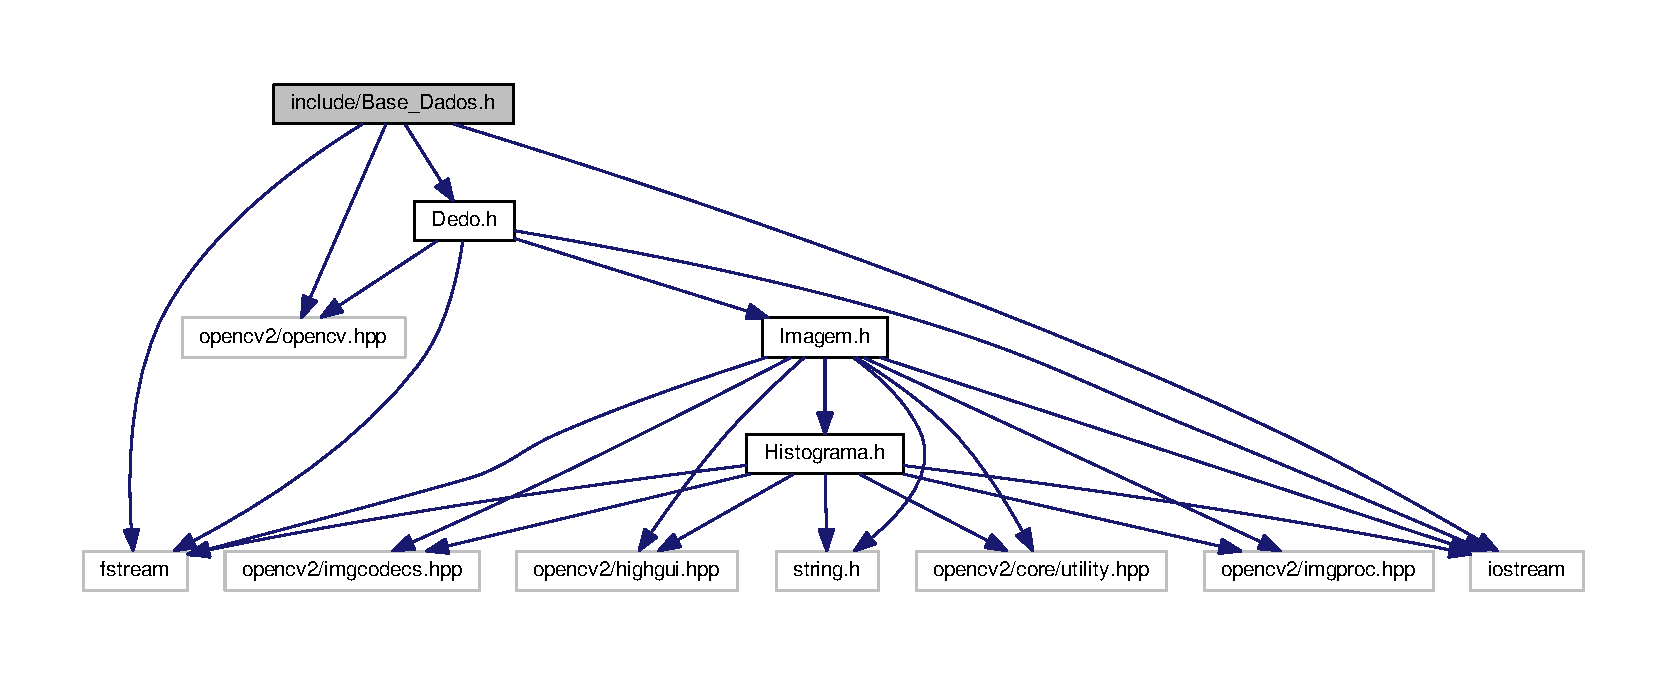
\includegraphics[width=350pt]{_base___dados_8h__incl}
\end{center}
\end{figure}
This graph shows which files directly or indirectly include this file\+:\nopagebreak
\begin{figure}[H]
\begin{center}
\leavevmode
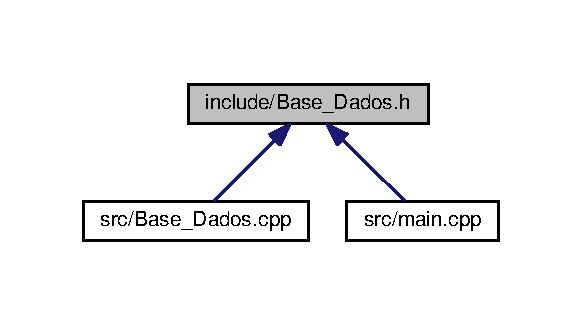
\includegraphics[width=280pt]{_base___dados_8h__dep__incl}
\end{center}
\end{figure}
\subsection*{Classes}
\begin{DoxyCompactItemize}
\item 
class \mbox{\hyperlink{classbase}{base}}
\begin{DoxyCompactList}\small\item\em Classe que implementa um objeto que é a base de dados que guarda informações sobre diversas impressões digitais. \end{DoxyCompactList}\end{DoxyCompactItemize}


\subsection{Detailed Description}
A base de dados é uma estrutura que armazena algumas impressões digitais em uma estrurura. 

\begin{DoxyAuthor}{Author}
Douglas Venâncio Filipe Pena Marco Antonio 
\end{DoxyAuthor}
\begin{DoxyDate}{Date}
2018-\/07-\/01 
\end{DoxyDate}

\hypertarget{_dedo_8h}{}\section{include/\+Dedo.h File Reference}
\label{_dedo_8h}\index{include/\+Dedo.\+h@{include/\+Dedo.\+h}}


Aquivo que implementa os metodos referentes a uma estrutura de objeto dedo.  


{\ttfamily \#include \char`\"{}opencv2/opencv.\+hpp\char`\"{}}\newline
{\ttfamily \#include $<$fstream$>$}\newline
{\ttfamily \#include $<$iostream$>$}\newline
{\ttfamily \#include \char`\"{}Imagem.\+h\char`\"{}}\newline
Include dependency graph for Dedo.\+h\+:\nopagebreak
\begin{figure}[H]
\begin{center}
\leavevmode
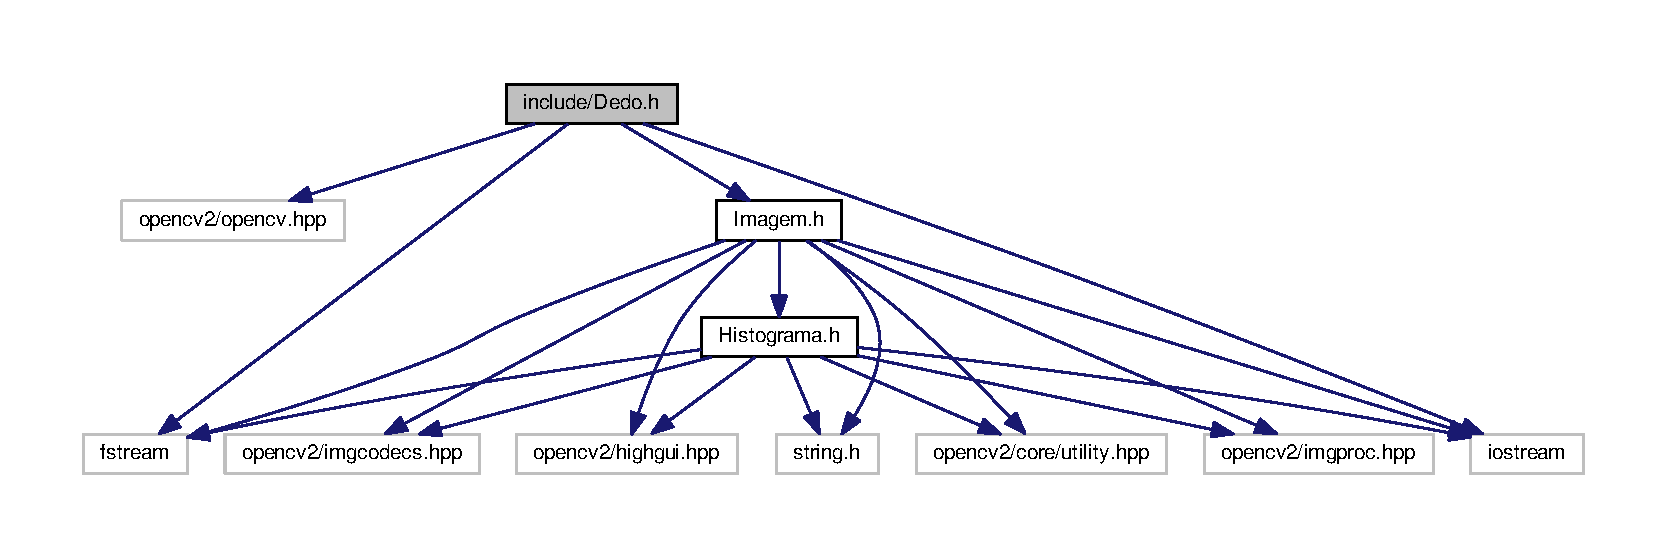
\includegraphics[width=350pt]{_dedo_8h__incl}
\end{center}
\end{figure}
This graph shows which files directly or indirectly include this file\+:\nopagebreak
\begin{figure}[H]
\begin{center}
\leavevmode
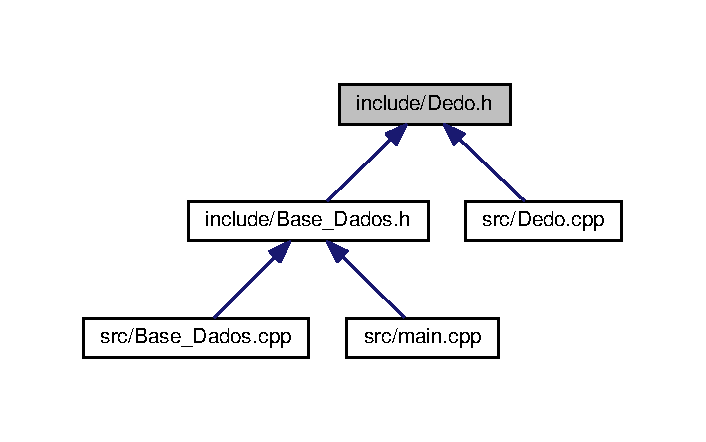
\includegraphics[width=339pt]{_dedo_8h__dep__incl}
\end{center}
\end{figure}
\subsection*{Classes}
\begin{DoxyCompactItemize}
\item 
class \mbox{\hyperlink{classdedo}{dedo}}
\begin{DoxyCompactList}\small\item\em Classe que implementa o objeto dedo, objeto esse que possui a imagem do dedo, o nome do dono do dedo e outros parâmeros. \end{DoxyCompactList}\end{DoxyCompactItemize}


\subsection{Detailed Description}
Aquivo que implementa os metodos referentes a uma estrutura de objeto dedo. 

\begin{DoxyAuthor}{Author}
Douglas Venâncio Filipe Pena Marco Antonio 
\end{DoxyAuthor}
\begin{DoxyDate}{Date}
2018-\/07-\/01 
\end{DoxyDate}

\hypertarget{_histograma_8h}{}\section{include/\+Histograma.h File Reference}
\label{_histograma_8h}\index{include/\+Histograma.\+h@{include/\+Histograma.\+h}}


Classe utilizada para manipulação do histograma.  


{\ttfamily \#include \char`\"{}opencv2/core/utility.\+hpp\char`\"{}}\newline
{\ttfamily \#include \char`\"{}opencv2/imgproc.\+hpp\char`\"{}}\newline
{\ttfamily \#include \char`\"{}opencv2/imgcodecs.\+hpp\char`\"{}}\newline
{\ttfamily \#include \char`\"{}opencv2/highgui.\+hpp\char`\"{}}\newline
{\ttfamily \#include $<$iostream$>$}\newline
{\ttfamily \#include $<$string.\+h$>$}\newline
{\ttfamily \#include $<$fstream$>$}\newline
Include dependency graph for Histograma.\+h\+:\nopagebreak
\begin{figure}[H]
\begin{center}
\leavevmode
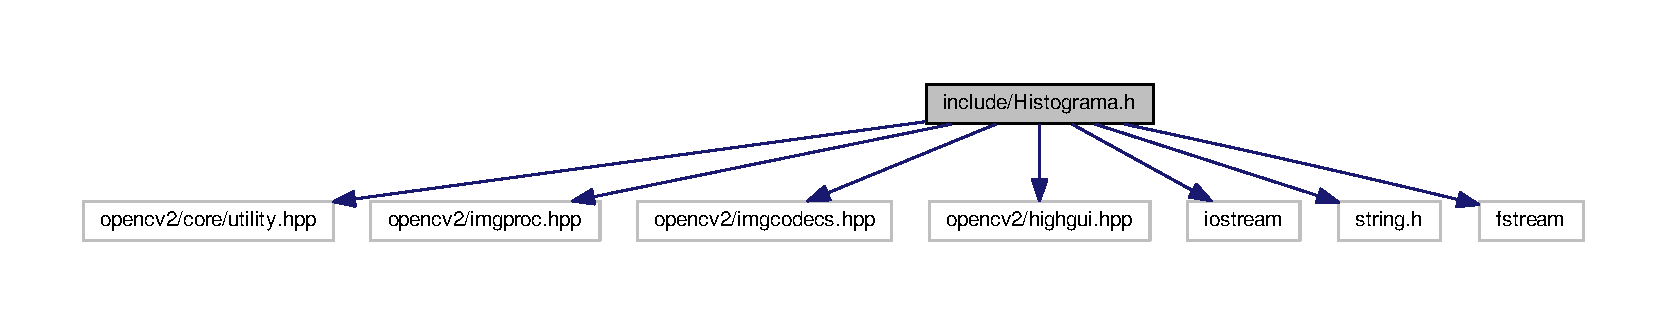
\includegraphics[width=350pt]{_histograma_8h__incl}
\end{center}
\end{figure}
This graph shows which files directly or indirectly include this file\+:\nopagebreak
\begin{figure}[H]
\begin{center}
\leavevmode
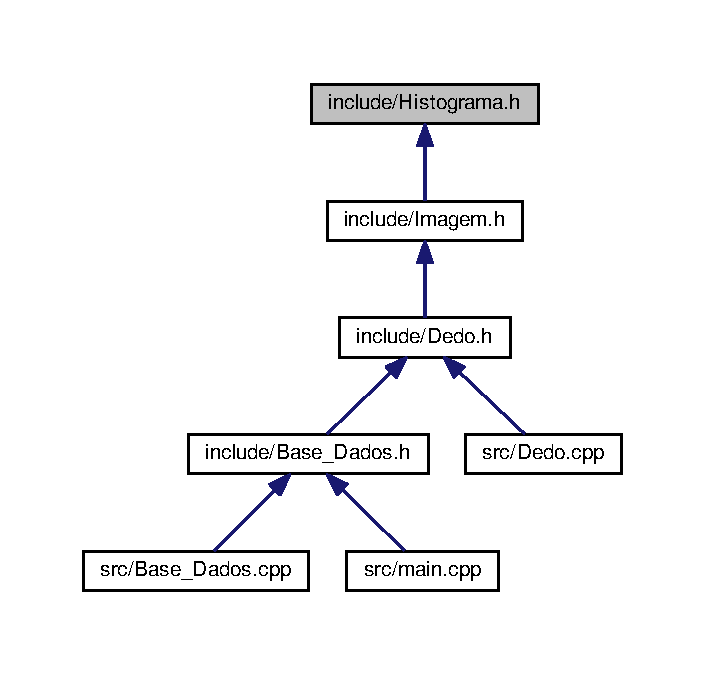
\includegraphics[width=339pt]{_histograma_8h__dep__incl}
\end{center}
\end{figure}
\subsection*{Classes}
\begin{DoxyCompactItemize}
\item 
class \mbox{\hyperlink{classhistograma}{histograma}}
\begin{DoxyCompactList}\small\item\em Classe que implementa o histograma de uma imagem. \end{DoxyCompactList}\end{DoxyCompactItemize}


\subsection{Detailed Description}
Classe utilizada para manipulação do histograma. 

\begin{DoxyAuthor}{Author}
Douglas Venâncio Filipe Pena Marco Antonio 
\end{DoxyAuthor}
\begin{DoxyDate}{Date}
2018-\/07-\/01 
\end{DoxyDate}

\hypertarget{_imagem_8h}{}\section{include/\+Imagem.h File Reference}
\label{_imagem_8h}\index{include/\+Imagem.\+h@{include/\+Imagem.\+h}}


Classe utilizada para o tratamento de imagens.  


{\ttfamily \#include \char`\"{}opencv2/core/utility.\+hpp\char`\"{}}\newline
{\ttfamily \#include \char`\"{}opencv2/imgproc.\+hpp\char`\"{}}\newline
{\ttfamily \#include \char`\"{}opencv2/imgcodecs.\+hpp\char`\"{}}\newline
{\ttfamily \#include \char`\"{}opencv2/highgui.\+hpp\char`\"{}}\newline
{\ttfamily \#include $<$iostream$>$}\newline
{\ttfamily \#include $<$string.\+h$>$}\newline
{\ttfamily \#include $<$fstream$>$}\newline
{\ttfamily \#include \char`\"{}Histograma.\+h\char`\"{}}\newline
Include dependency graph for Imagem.\+h\+:\nopagebreak
\begin{figure}[H]
\begin{center}
\leavevmode
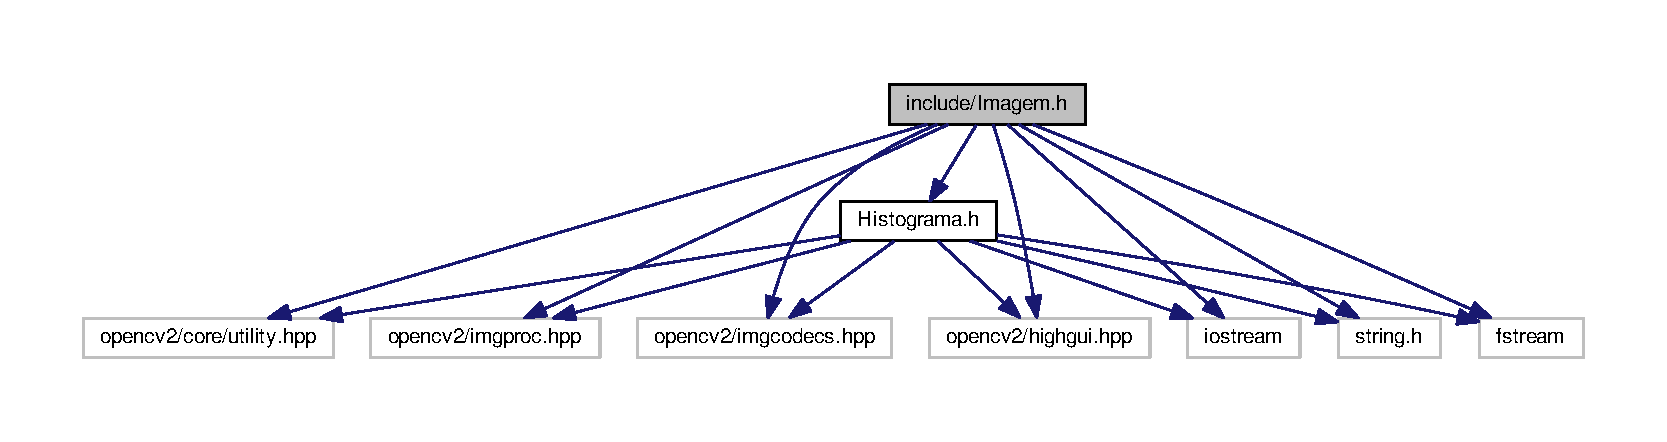
\includegraphics[width=350pt]{_imagem_8h__incl}
\end{center}
\end{figure}
This graph shows which files directly or indirectly include this file\+:\nopagebreak
\begin{figure}[H]
\begin{center}
\leavevmode
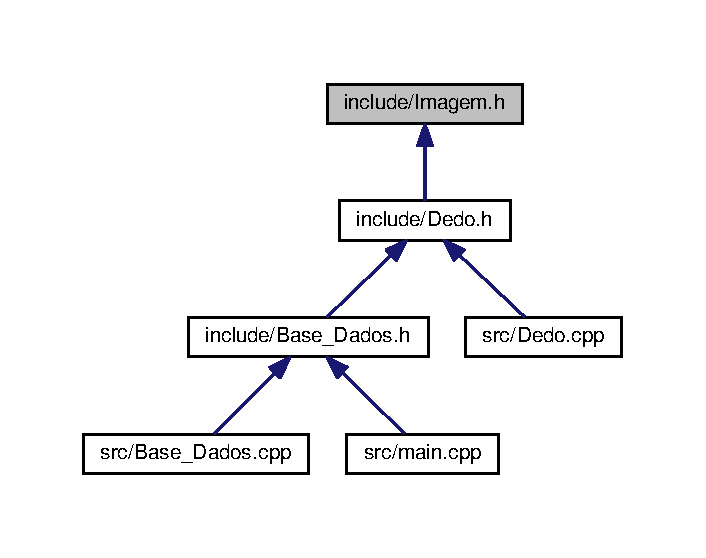
\includegraphics[width=339pt]{_imagem_8h__dep__incl}
\end{center}
\end{figure}
\subsection*{Classes}
\begin{DoxyCompactItemize}
\item 
class \mbox{\hyperlink{classimagem}{imagem}}
\begin{DoxyCompactList}\small\item\em Classe que implementa uma imagem e as possiveis operações feitas nela. \end{DoxyCompactList}\end{DoxyCompactItemize}


\subsection{Detailed Description}
Classe utilizada para o tratamento de imagens. 

\begin{DoxyAuthor}{Author}
Douglas Venâncio Filipe Pena Marco Antonio 
\end{DoxyAuthor}
\begin{DoxyDate}{Date}
2018-\/07-\/01 
\end{DoxyDate}

\hypertarget{_base___dados_8cpp}{}\section{src/\+Base\+\_\+\+Dados.cpp File Reference}
\label{_base___dados_8cpp}\index{src/\+Base\+\_\+\+Dados.\+cpp@{src/\+Base\+\_\+\+Dados.\+cpp}}


A base de dados é uma estrutura que armazena algumas impressões digitais em uma estrurura.  


{\ttfamily \#include \char`\"{}../include/\+Base\+\_\+\+Dados.\+h\char`\"{}}\newline
{\ttfamily \#include \char`\"{}opencv2/opencv.\+hpp\char`\"{}}\newline
{\ttfamily \#include $<$fstream$>$}\newline
{\ttfamily \#include $<$iostream$>$}\newline
Include dependency graph for Base\+\_\+\+Dados.\+cpp\+:\nopagebreak
\begin{figure}[H]
\begin{center}
\leavevmode
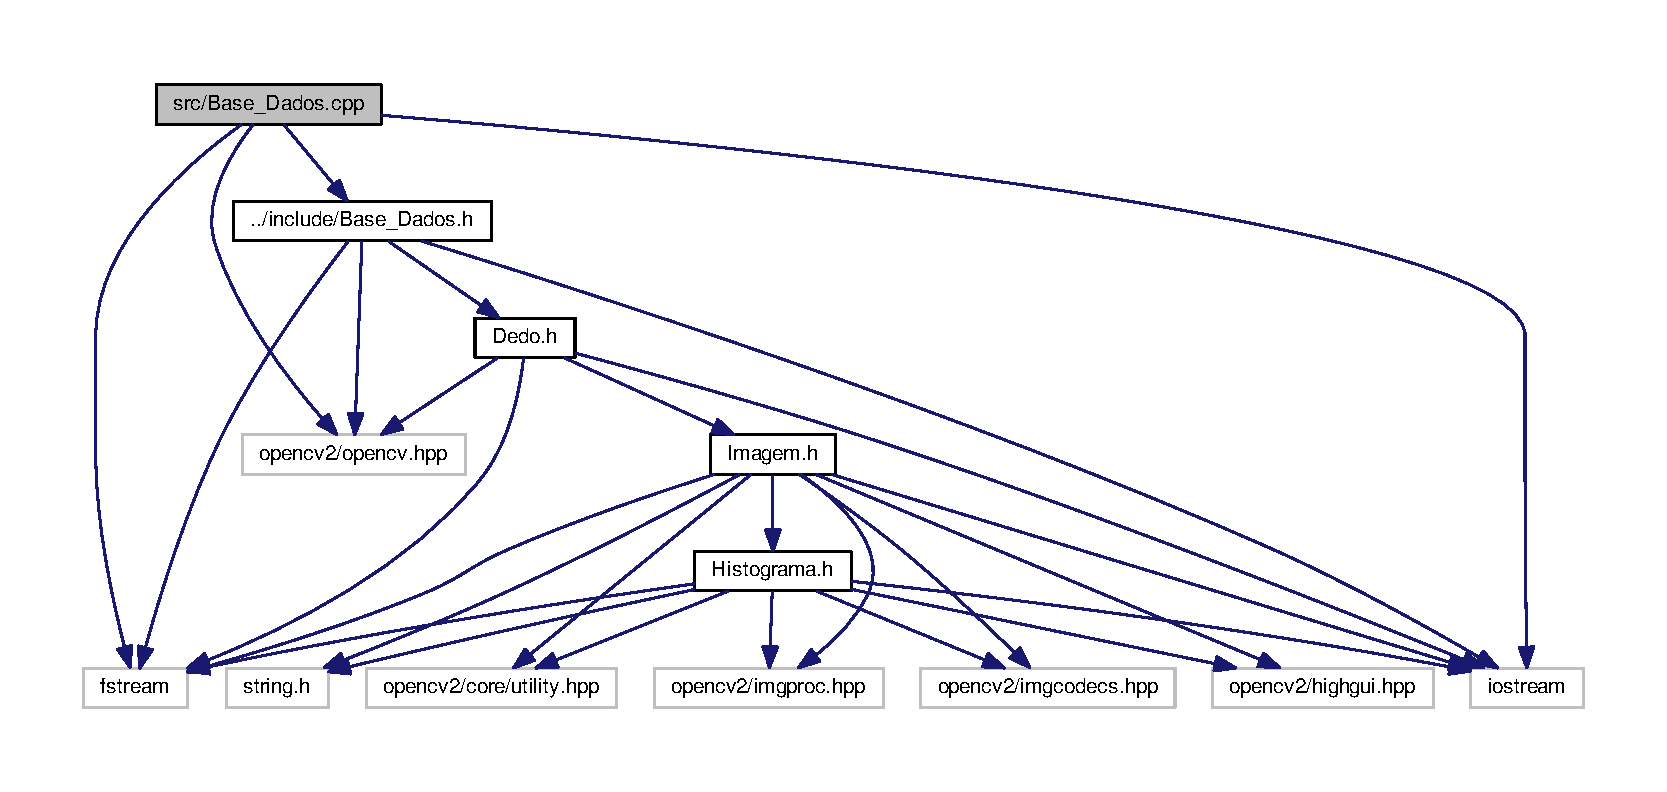
\includegraphics[width=350pt]{_base___dados_8cpp__incl}
\end{center}
\end{figure}


\subsection{Detailed Description}
A base de dados é uma estrutura que armazena algumas impressões digitais em uma estrurura. 

\begin{DoxyAuthor}{Author}
Douglas Venâncio Filipe Pena Marco Antonio 
\end{DoxyAuthor}
\begin{DoxyDate}{Date}
2018-\/07-\/01 
\end{DoxyDate}

\hypertarget{_dedo_8cpp}{}\section{src/\+Dedo.cpp File Reference}
\label{_dedo_8cpp}\index{src/\+Dedo.\+cpp@{src/\+Dedo.\+cpp}}


Aquivo que implementa os metodos referentes a uma estrutura de objeto dedo.  


{\ttfamily \#include \char`\"{}opencv2/opencv.\+hpp\char`\"{}}\newline
{\ttfamily \#include $<$fstream$>$}\newline
{\ttfamily \#include $<$iostream$>$}\newline
{\ttfamily \#include \char`\"{}../include/\+Dedo.\+h\char`\"{}}\newline
Include dependency graph for Dedo.\+cpp\+:\nopagebreak
\begin{figure}[H]
\begin{center}
\leavevmode
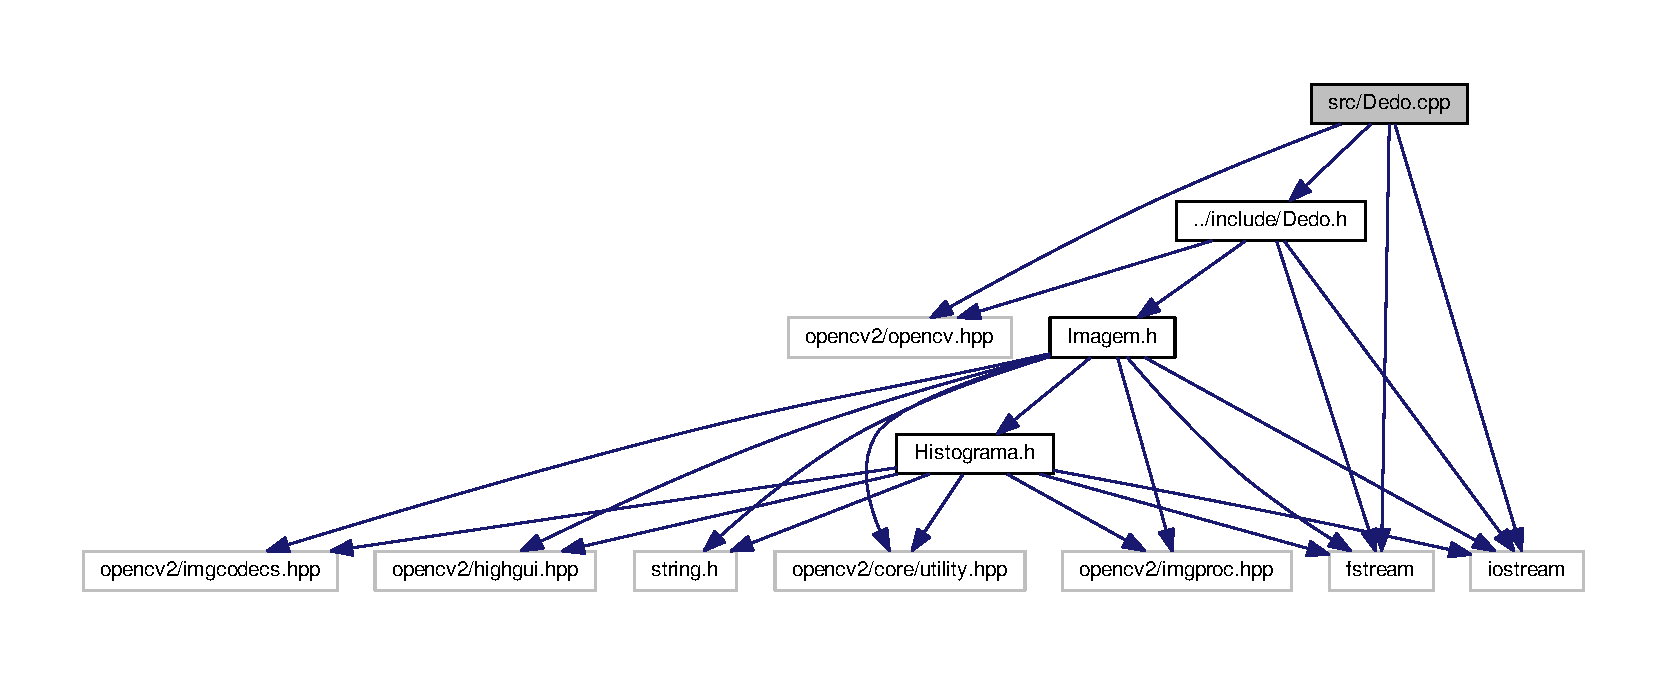
\includegraphics[width=350pt]{_dedo_8cpp__incl}
\end{center}
\end{figure}


\subsection{Detailed Description}
Aquivo que implementa os metodos referentes a uma estrutura de objeto dedo. 

\begin{DoxyAuthor}{Author}
Douglas Venâncio Filipe Pena Marco Antonio 
\end{DoxyAuthor}
\begin{DoxyDate}{Date}
2018-\/07-\/01 
\end{DoxyDate}

\hypertarget{main_8cpp}{}\section{src/main.cpp File Reference}
\label{main_8cpp}\index{src/main.\+cpp@{src/main.\+cpp}}


Classe principal do trabalho.  


{\ttfamily \#include \char`\"{}opencv2/core/utility.\+hpp\char`\"{}}\newline
{\ttfamily \#include \char`\"{}opencv2/imgproc.\+hpp\char`\"{}}\newline
{\ttfamily \#include \char`\"{}opencv2/imgcodecs.\+hpp\char`\"{}}\newline
{\ttfamily \#include \char`\"{}opencv2/highgui.\+hpp\char`\"{}}\newline
{\ttfamily \#include $<$opencv2/opencv.\+hpp$>$}\newline
{\ttfamily \#include \char`\"{}../include/\+Base\+\_\+\+Dados.\+h\char`\"{}}\newline
{\ttfamily \#include $<$iostream$>$}\newline
Include dependency graph for main.\+cpp\+:\nopagebreak
\begin{figure}[H]
\begin{center}
\leavevmode
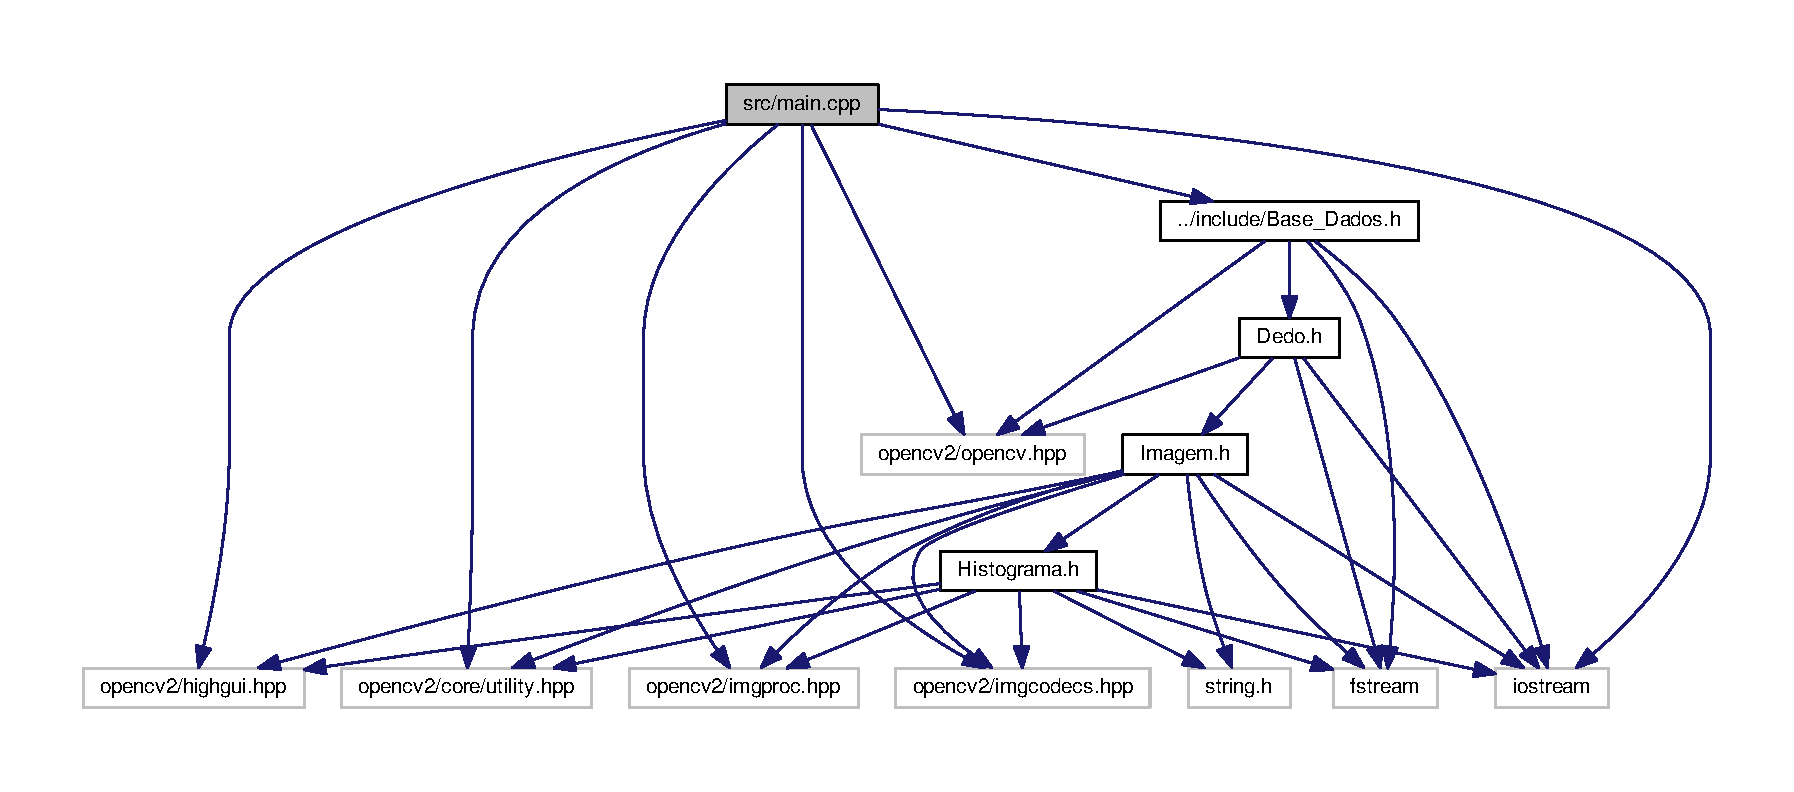
\includegraphics[width=350pt]{main_8cpp__incl}
\end{center}
\end{figure}
\subsection*{Functions}
\begin{DoxyCompactItemize}
\item 
\mbox{\Hypertarget{main_8cpp_a217dbf8b442f20279ea00b898af96f52}\label{main_8cpp_a217dbf8b442f20279ea00b898af96f52}} 
int {\bfseries main} (int argc, const char $\ast$$\ast$argv)
\end{DoxyCompactItemize}
\subsection*{Variables}
\begin{DoxyCompactItemize}
\item 
const char $\ast$ {\bfseries keys}
\end{DoxyCompactItemize}


\subsection{Detailed Description}
Classe principal do trabalho. 

\begin{DoxyAuthor}{Author}
Douglas Venâncio Filipe Pena Marco Antonio 
\end{DoxyAuthor}
\begin{DoxyDate}{Date}
2018-\/07-\/01 
\end{DoxyDate}


\subsection{Variable Documentation}
\mbox{\Hypertarget{main_8cpp_ad369b0cdd85ef6d6db7446dba8b57a27}\label{main_8cpp_ad369b0cdd85ef6d6db7446dba8b57a27}} 
\index{main.\+cpp@{main.\+cpp}!keys@{keys}}
\index{keys@{keys}!main.\+cpp@{main.\+cpp}}
\subsubsection{\texorpdfstring{keys}{keys}}
{\footnotesize\ttfamily const char$\ast$ keys}

{\bfseries Initial value\+:}
\begin{DoxyCode}
\DoxyCodeLine{=}
\DoxyCodeLine{    \{}
\DoxyCodeLine{        \textcolor{stringliteral}{"\{help h||\}\{@image |../src/img/d1\_5.png|input image name\}\{@image |../src/img/110\_8.tif|input image name\}"}\}}
\end{DoxyCode}

%--- End generated contents ---

% Index
\backmatter
\newpage
\phantomsection
\clearemptydoublepage
\addcontentsline{toc}{chapter}{\indexname}
\printindex

\end{document}
